\section{实验结果}

\subsection{加速度计标定与补偿结果}
为建立加速度计六位置静态标定模型，分别将IMU置于
$X$上、$X$下、$Y$上、$Y$下、$Z$上和$Z$下六种姿态，
在各姿态对应的静态稳定区间内提取三轴比力观测值，
并计算各轴比力的时间平均值，结果如表\ref{tab:means}所示。

理想情况下，当IMU某一敏感轴正向或反向与当地重力方向对准时，
该轴应分别测得约$+g$和$-g$的比力，
其余两个敏感轴的比力应接近零。
因此，六个位置的三轴比力均值既反映了加速度计对重力的响应，
也为后续零偏、比例因子及交轴耦合误差的联合估计提供观测数据。
\begin{table}[htbp]\centering\small
    \caption{选定静态区间三轴比力均值（m/s$^2$）}\label{tab:means}
    \begin{tabular}{crrr}\toprule
    位置&$\overline f_x$&$\overline f_y$&$\overline f_z$\\\midrule
    $X$上&9.812176&0.005709&0.003536\\
    $X$下&-9.818956&0.032958&-0.022392\\
    $Y$上&0.003922&9.833014&0.062776\\
    $Y$下&-0.017429&-9.798641&-0.080701\\
    $Z$上&-0.019804&-0.056923&9.807740\\
    $Z$下&0.012681&0.096186&-9.825926\\\bottomrule
    \end{tabular}
\end{table}
从表中可以看出，六个位置的主敏感轴比力均值均接近
$+g$或$-g$，与六位置静态标定的理论预期基本一致。
与此同时，非主敏感轴分量并非严格为零，
其绝对值最大达到$0.096186~\mathrm{m/s^2}$，
约为当地重力加速度的$0.98\%$。
此外，同一敏感轴在正、反两个位置测得的比力也并非严格等幅反号。

上述偏差可能与加速度计零偏、比例因子误差、交轴耦合、
IMU安装不正交以及转台姿态定位误差等因素有关。
因此，需要利用六个位置的全部三轴观测信息，
通过建立的误差模型进行联合估计，
而不能仅根据各轴正、反位置的比力差直接确定标定参数。

将表\ref{tab:means}中的六位置三轴比力均值代入式
\eqref{eq:accls}，采用最小二乘法联合估计加速度计的
零偏、比例因子及交轴耦合参数，结果如表\ref{tab:accparam}所示。
比例及交轴系数以ppm表达，$1~\mathrm{ppm}=10^{-6}$；
$1~\mathrm{mGal}=10^{-5}$~m/s$^2$。

\begin{table}[htbp]\centering\small
    \caption{加速度计零偏与比例因子误差}\label{tab:accparam}
    \begin{tabular}{crrr}\toprule
    轴&零偏/(m/s$^2$)&零偏/mGal&比例误差/ppm\\\midrule
    $X$&-0.00456837&-456.837&2241.114\\
    $Y$&0.01871715&1871.715&2267.775\\
    $Z$&-0.00916109&-916.109&2370.495\\\bottomrule
    \end{tabular}
\end{table}

六项交轴耦合误差为

\begin{equation}
\widehat{\matr M}_a=10^{-6}
\begin{bmatrix}
0&1090.058&-1658.488\\-1391.169&0&-7816.797\\1323.753&7325.073&0
\end{bmatrix}.
\label{eq:crossresult}\end{equation}
完整响应矩阵条件数为1.000662，不存在明显病态放大。$Y$与$Z$之间交轴项最大，约为$7\sim8\times10^{-3}$。这些是给定六位置理想方向下的有效参数，可能吸收传感器不正交、安装不准和转台摆放误差。

\subsubsection{补偿前后对比}
定义各位置的补偿前、后均值残差：
\begin{equation}
    \matr e_p^{\rm raw}=\overline{\widetilde{\matr f}}_p-\matr f_p^{\rm ref},\qquad
    \matr e_p^{\rm com}=\overline{\widehat{\matr f}}_p-\matr f_p^{\rm ref}.
\end{equation}

图\ref{fig:accx}至图\ref{fig:accz}叠加展示每秒平均比力残差，时间范围统一为记录开始后的0-75~s。减参考值只改变纵轴原点，两条曲线使用相同时间分组；可见灰色区为未参与拟合的起始5~s。统计量仍在首尾各去5~s后的完整有效区间内计算，曲线每秒平均不参与参数拟合。

\begin{figure}[htbp]\centering
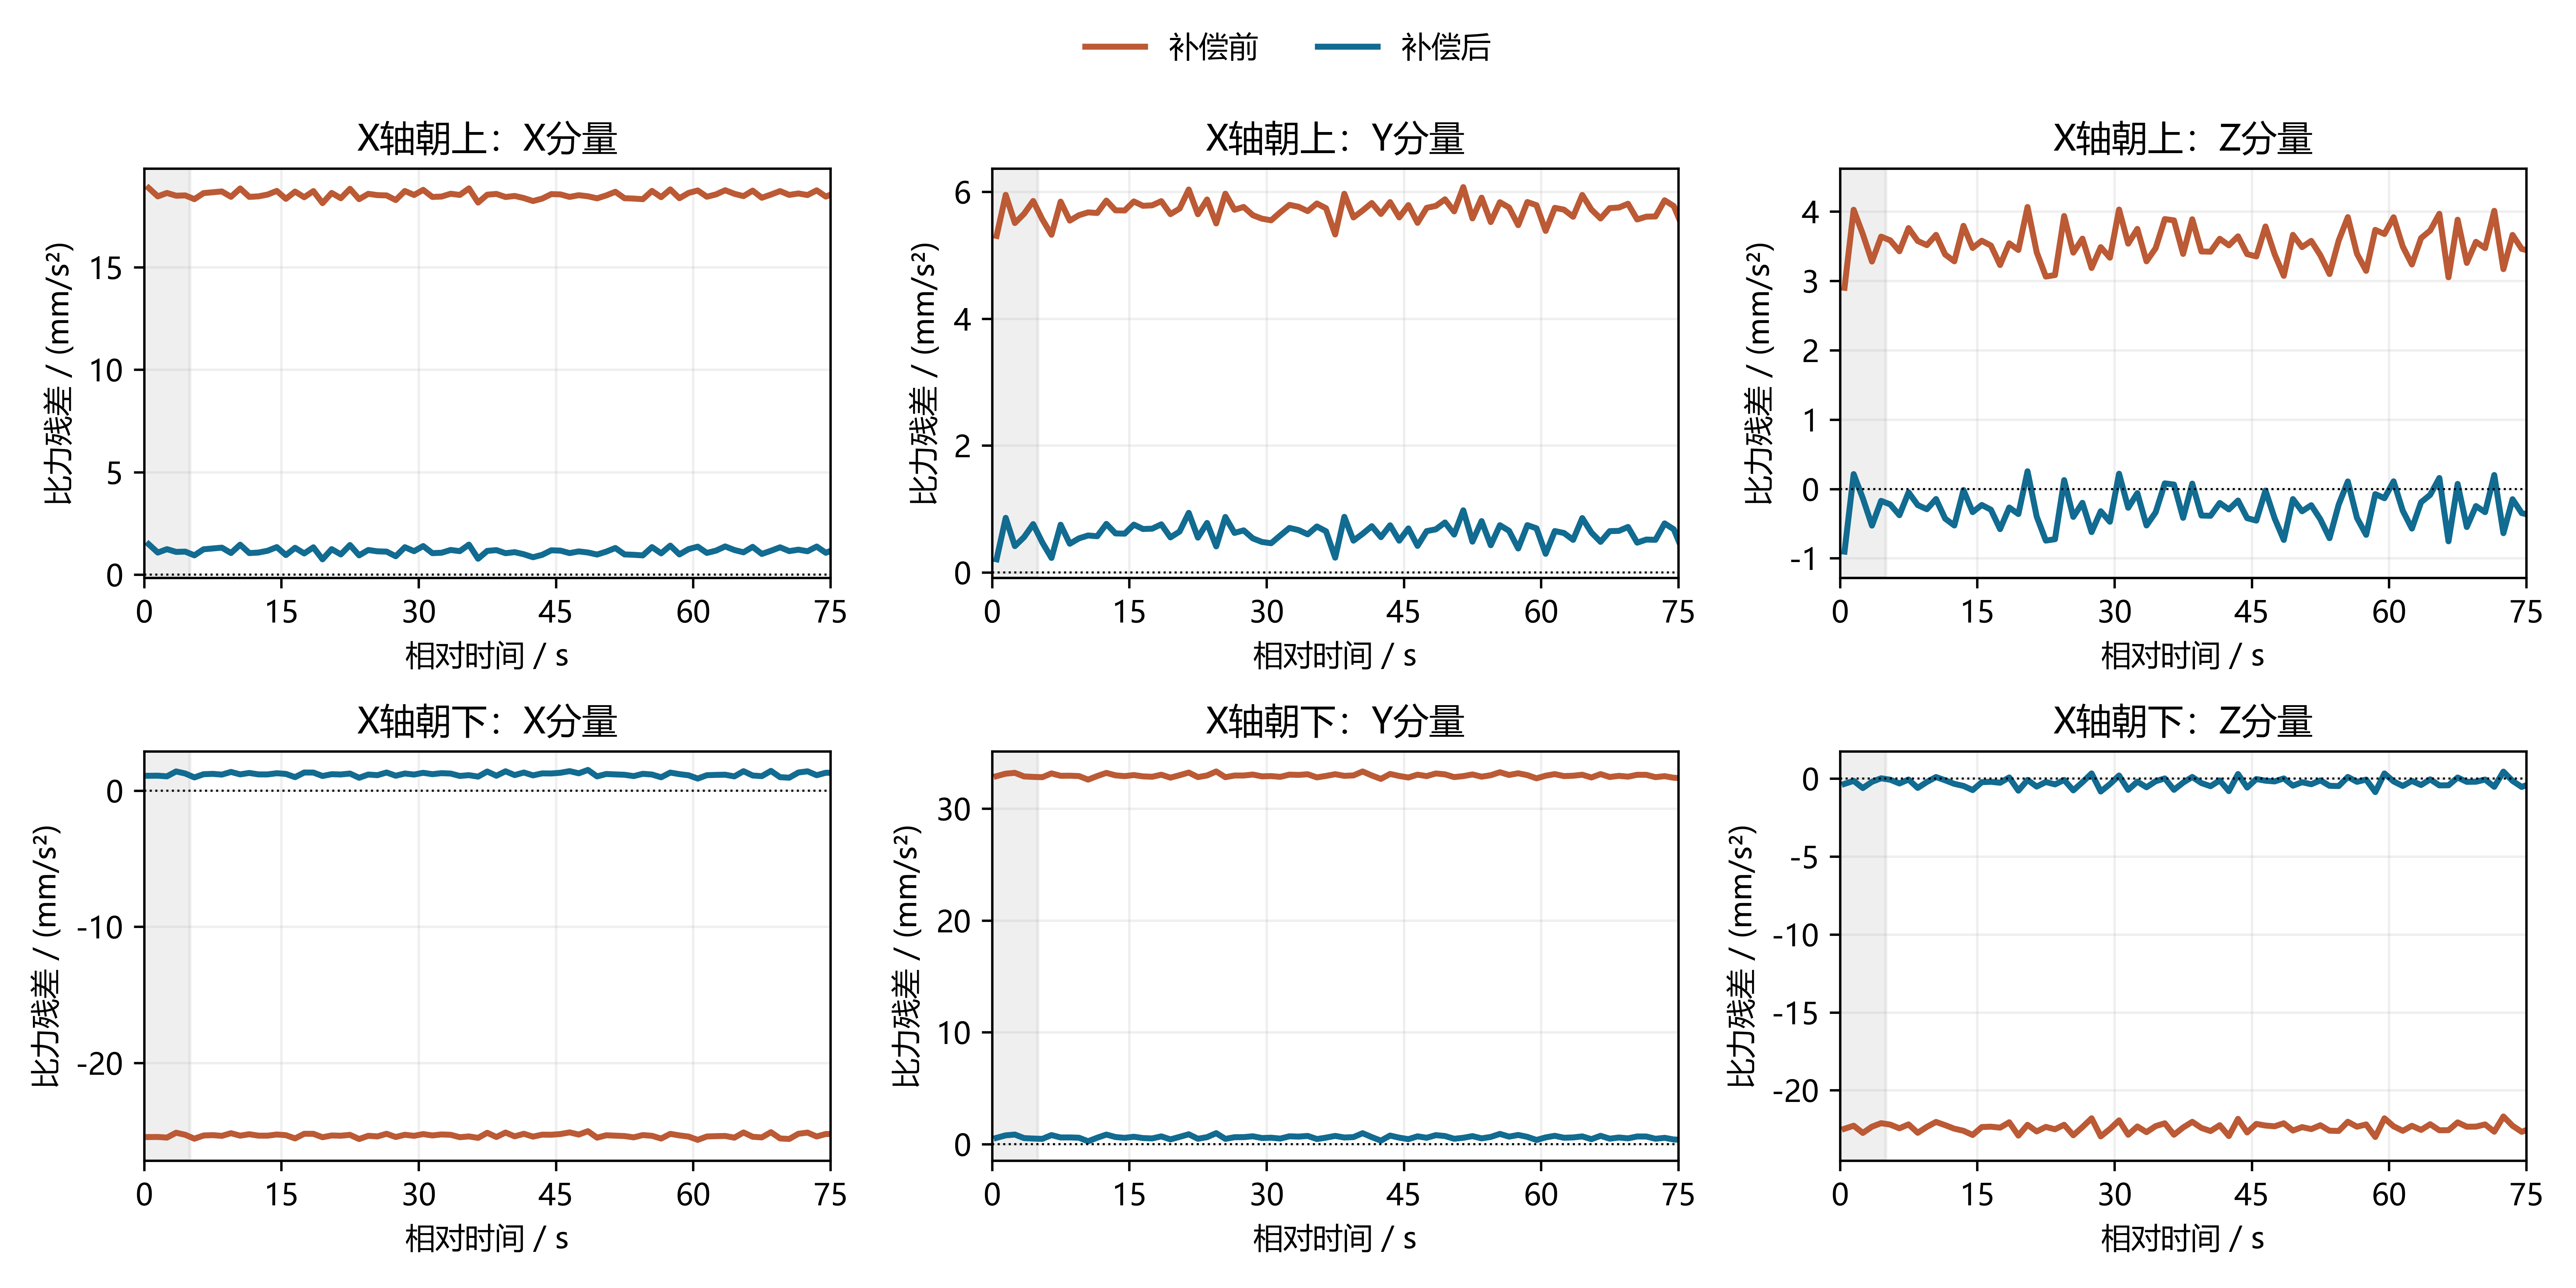
\includegraphics[width=0.95\textwidth]{acc_compensation_x.png}
\caption{$X$轴朝上/朝下时三轴比力残差补偿前后对比（每秒平均）}\label{fig:accx}
\end{figure}
图\ref{fig:accx}中主轴$X$分量的正负输入偏差得到校正，非主轴$Y$、$Z$分量也向零残差靠近，说明完整矩阵补偿同时处理主轴比例误差和交轴响应。

\begin{figure}[htbp]\centering
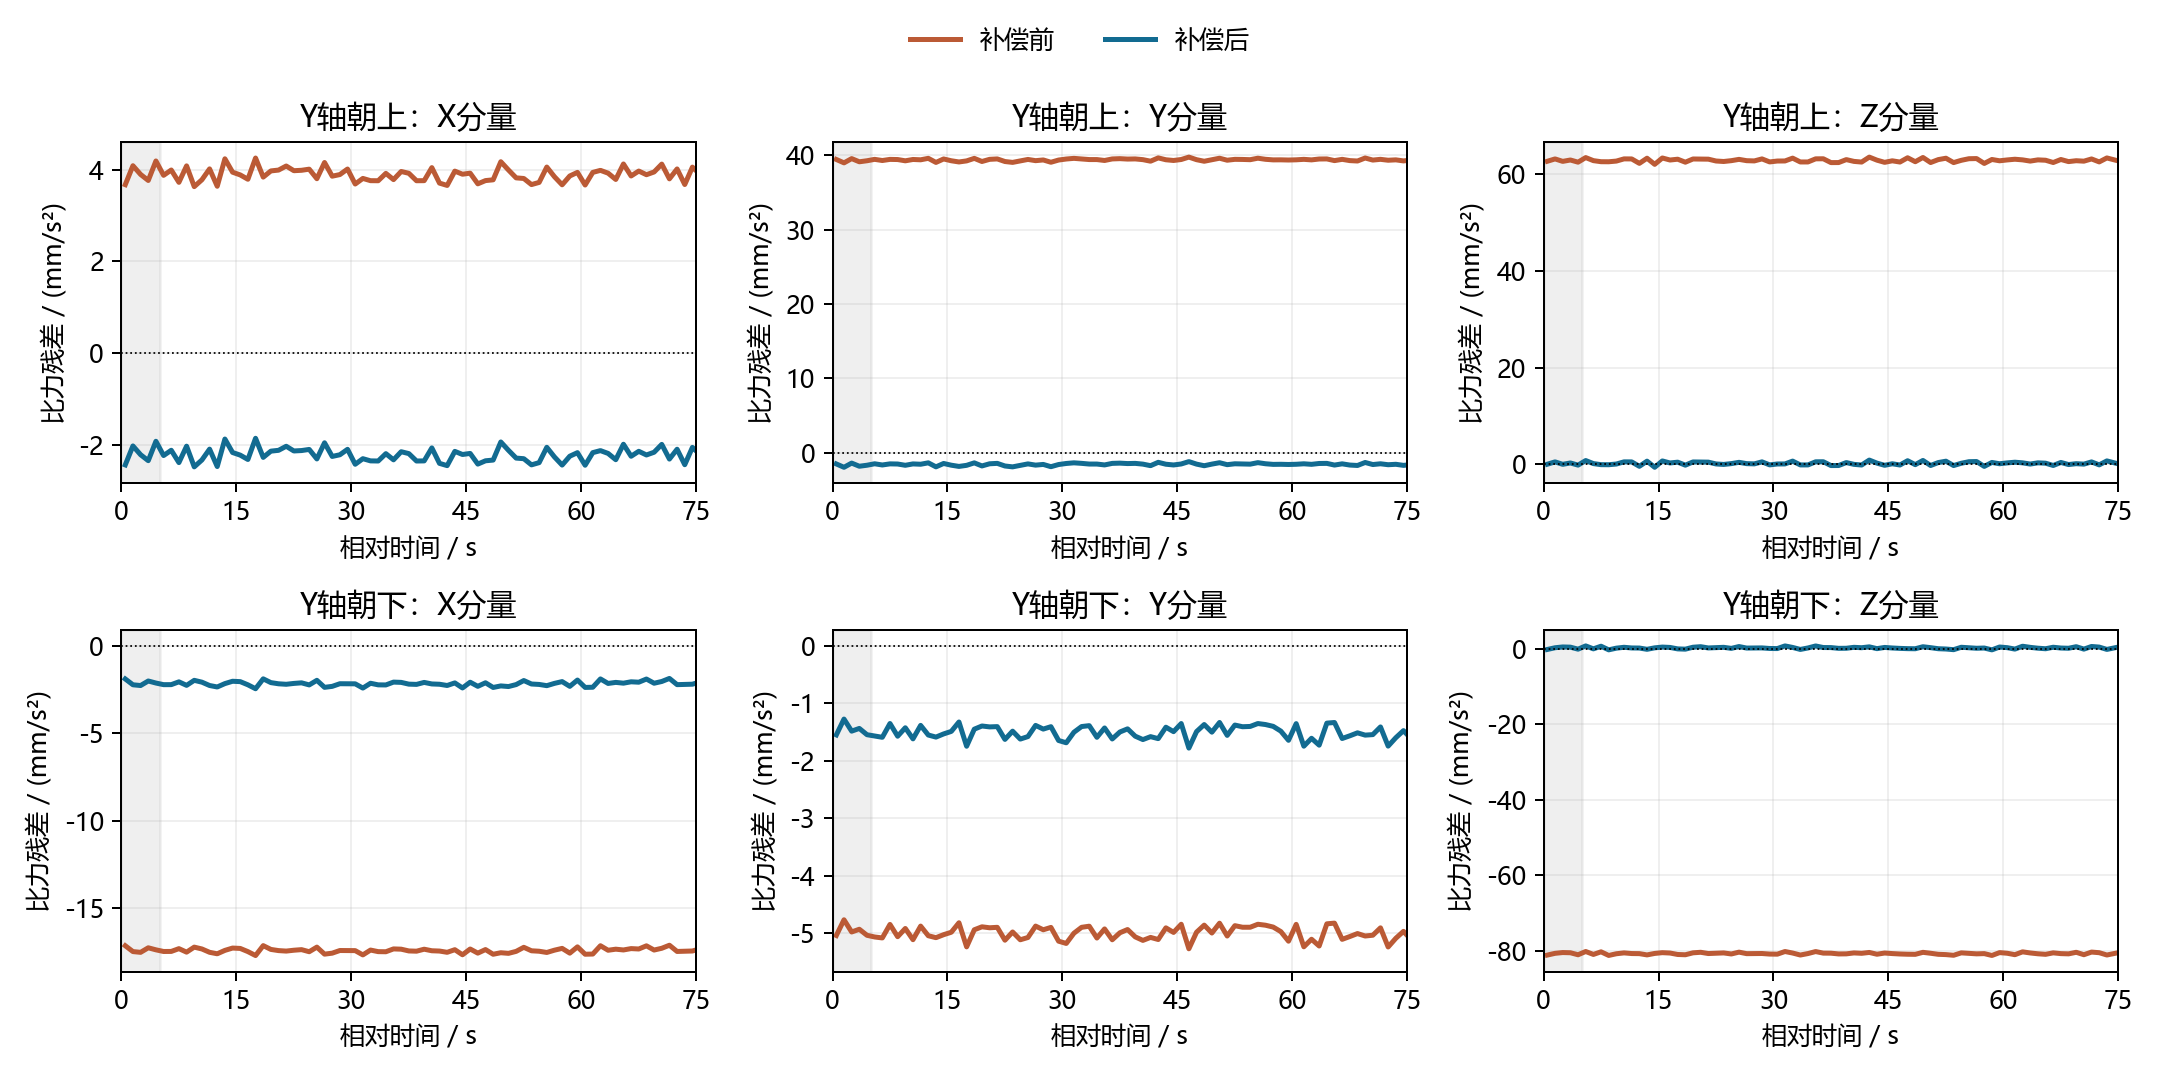
\includegraphics[width=0.95\textwidth]{acc_compensation_y.png}
\caption{$Y$轴朝上/朝下时三轴比力残差补偿前后对比（每秒平均）}\label{fig:accy}
\end{figure}
图\ref{fig:accy}中$Z$分量在两种姿态下的较大偏差明显减小，与较大的$Y$到$Z$交轴系数一致；$X$分量仍有小幅共同偏移，反映六位置线性模型的残余不一致。

\begin{figure}[htbp]\centering
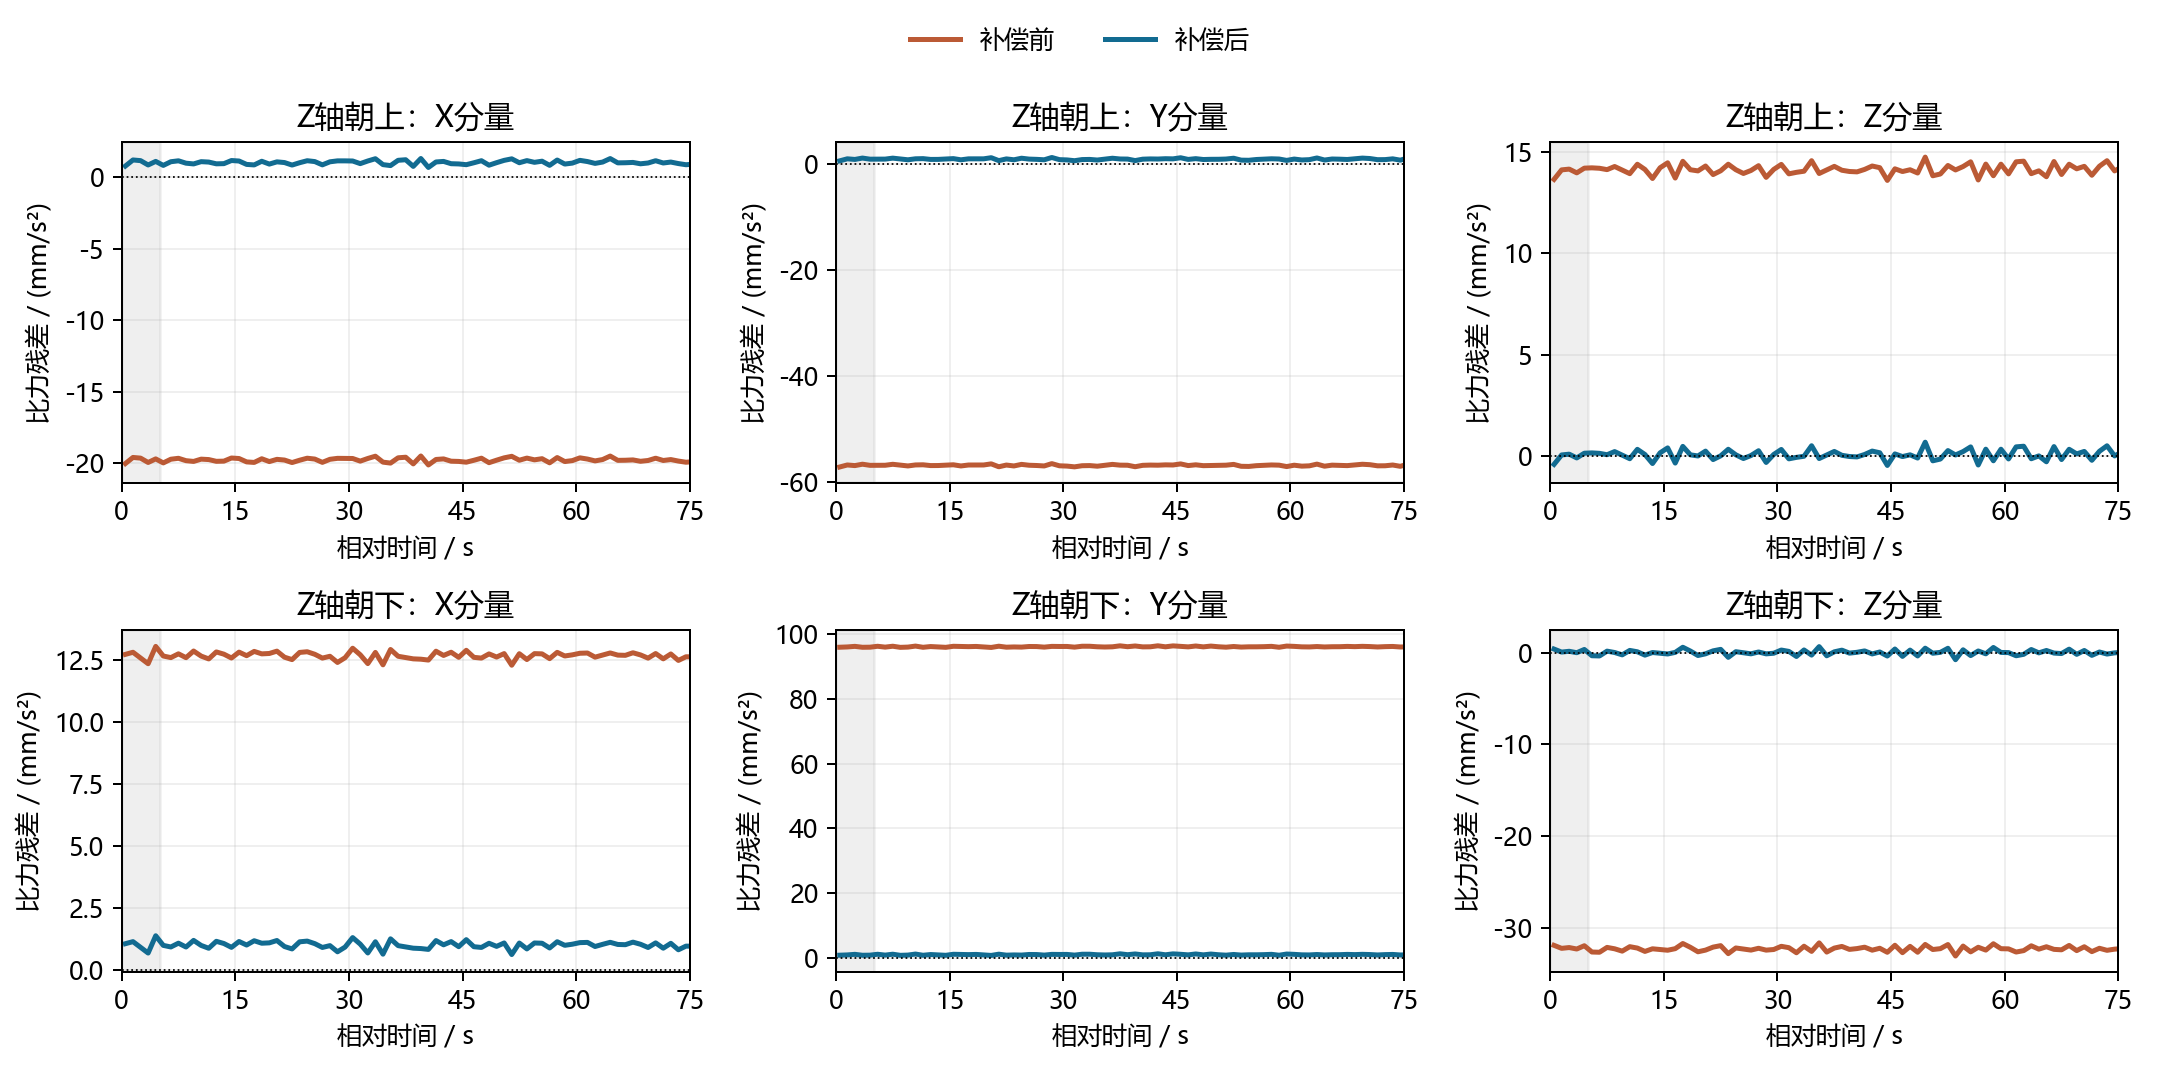
\includegraphics[width=0.95\textwidth]{acc_compensation_z.png}
\caption{$Z$轴朝上/朝下时三轴比力残差补偿前后对比（每秒平均）}\label{fig:accz}
\end{figure}
图\ref{fig:accz}显示$Z$输入引起的$Y$交轴偏差得到明显抑制，但补偿后曲线仍有随机起伏。参数校正主要移除系统偏差，并不能直接滤除白噪声。

\begin{figure}[htbp]\centering
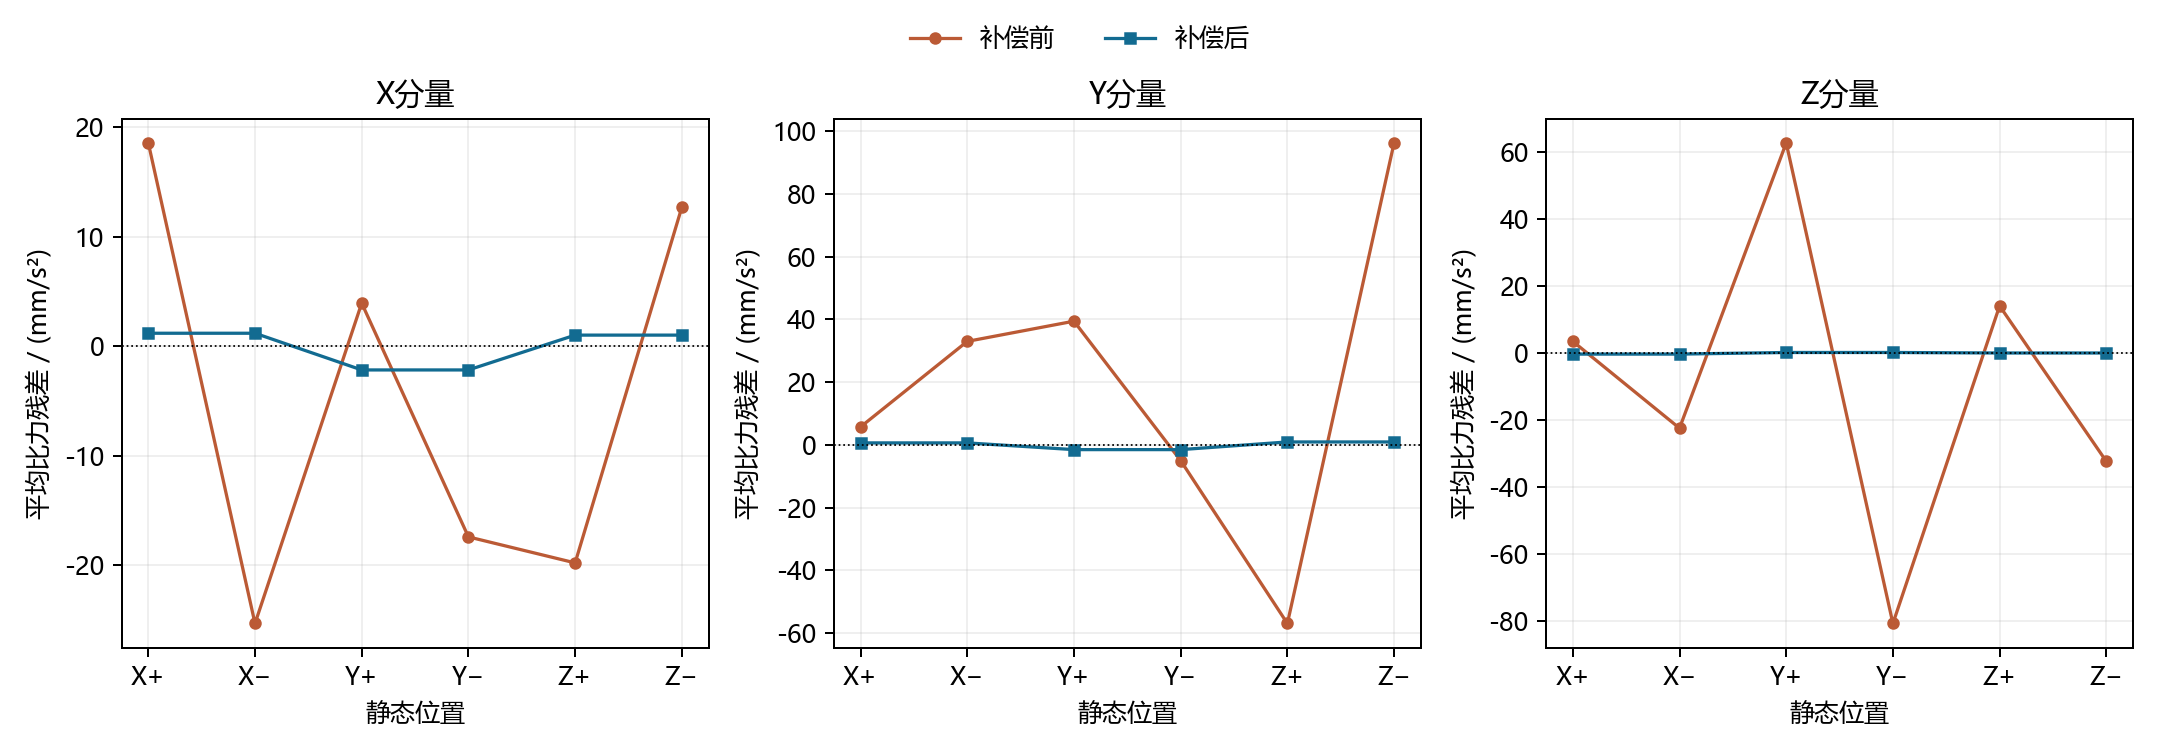
\includegraphics[width=0.95\textwidth]{acc_mean_residuals.png}
\caption{六位置三轴平均比力残差补偿前后对比}\label{fig:accmean}
\end{figure}
图\ref{fig:accmean}横轴依次为$X+$、$X-$、$Y+$、$Y-$、$Z+$、$Z-$，正负号表示对应轴朝上和朝下；三个子图分别比较$X$、$Y$、$Z$分量。每个点为完整有效静态区间的平均比力减去理想输入，连线仅辅助比较离散位置。补偿后残差整体靠近零，说明六位置间的系统偏差明显减小，但仍存在少量共同偏移。

\FloatBarrier
\begin{table}[htbp]\centering\small
\caption{六位置均值残差的跨位置RMS（mm/s$^2$）}\label{tab:accrms}
    \begin{tabular}{crrr}\toprule
    轴&补偿前&补偿后&降低比例/\%\\\midrule
    $X$&17.6004&1.5418&91.24\\
    $Y$&50.3126&1.0878&97.84\\
    $Z$&45.1125&0.2023&99.55\\\bottomrule
    \end{tabular}
\end{table}
表\ref{tab:accrms}采用$\sqrt{\sum_{p=1}^6 e_{p,i}^2/6}$，衡量六位置均值与理想输入的符合程度。补偿后18个均值残差的最大绝对值为0.002178~m/s$^2$，出现在$Y$上/下位置的$X$分量。不同位置对仍有共同偏移，说明线性模型不能完全解释位置间的不一致。

均值偏差减小不代表白噪声同步降低。以$Z$下位置的$Y$分量为例，逐历元对零输入RMS由0.109595降至0.052118~m/s$^2$，但去均值标准差仅由0.052530变为0.052111~m/s$^2$。改善主要来自消除系统偏差。


\subsection{陀螺标定与补偿结果}
\begin{table}[htbp]\centering\small
\caption{陀螺积分窗与原始积分角（GPS周2440）}\label{tab:windows}
    \begin{tabular}{crrrr}\toprule
    转动&首记录周内秒&末记录周内秒&$N\Delta t$/s&$\Theta$/($^\circ$)\\\midrule
    $X+$&290446.880&290486.930&40.055&359.800006\\
    $X-$&290743.615&290783.665&40.055&-359.966192\\
    $Y+$&292418.350&292458.400&40.055&359.806083\\
    $Y-$&292355.055&292395.105&40.055&-359.930159\\
    $Z+$&291493.125&291533.170&40.050&359.761934\\
    $Z-$&291557.285&291597.330&40.050&-359.881620\\\bottomrule
    \end{tabular}
\end{table}
积分时长按样本数计，比首末时间差多一个采样周期，因为每条数据对应一个增量。三轴正反转样本数分别为8011、8011、8010，轴内严格等长。

\begin{table}[htbp]\centering\small
\caption{陀螺静态零偏与角位置法比例因子误差}\label{tab:gyroparam}
    \begin{tabular}{crrrr}\toprule
    轴&朝上均值/($^\circ$/h)&朝下均值/($^\circ$/h)&零偏/($^\circ$/h)&比例误差/ppm\\\midrule
    $X$&6.134493&-8.072591&-0.969049&-324.725\\
    $Y$&7.746794&-6.359077&0.693858&-366.331\\
    $Z$&4.680487&-5.541972&-0.430742&-495.064\\\bottomrule
    \end{tabular}
\end{table}

\begin{figure}[htbp]\centering
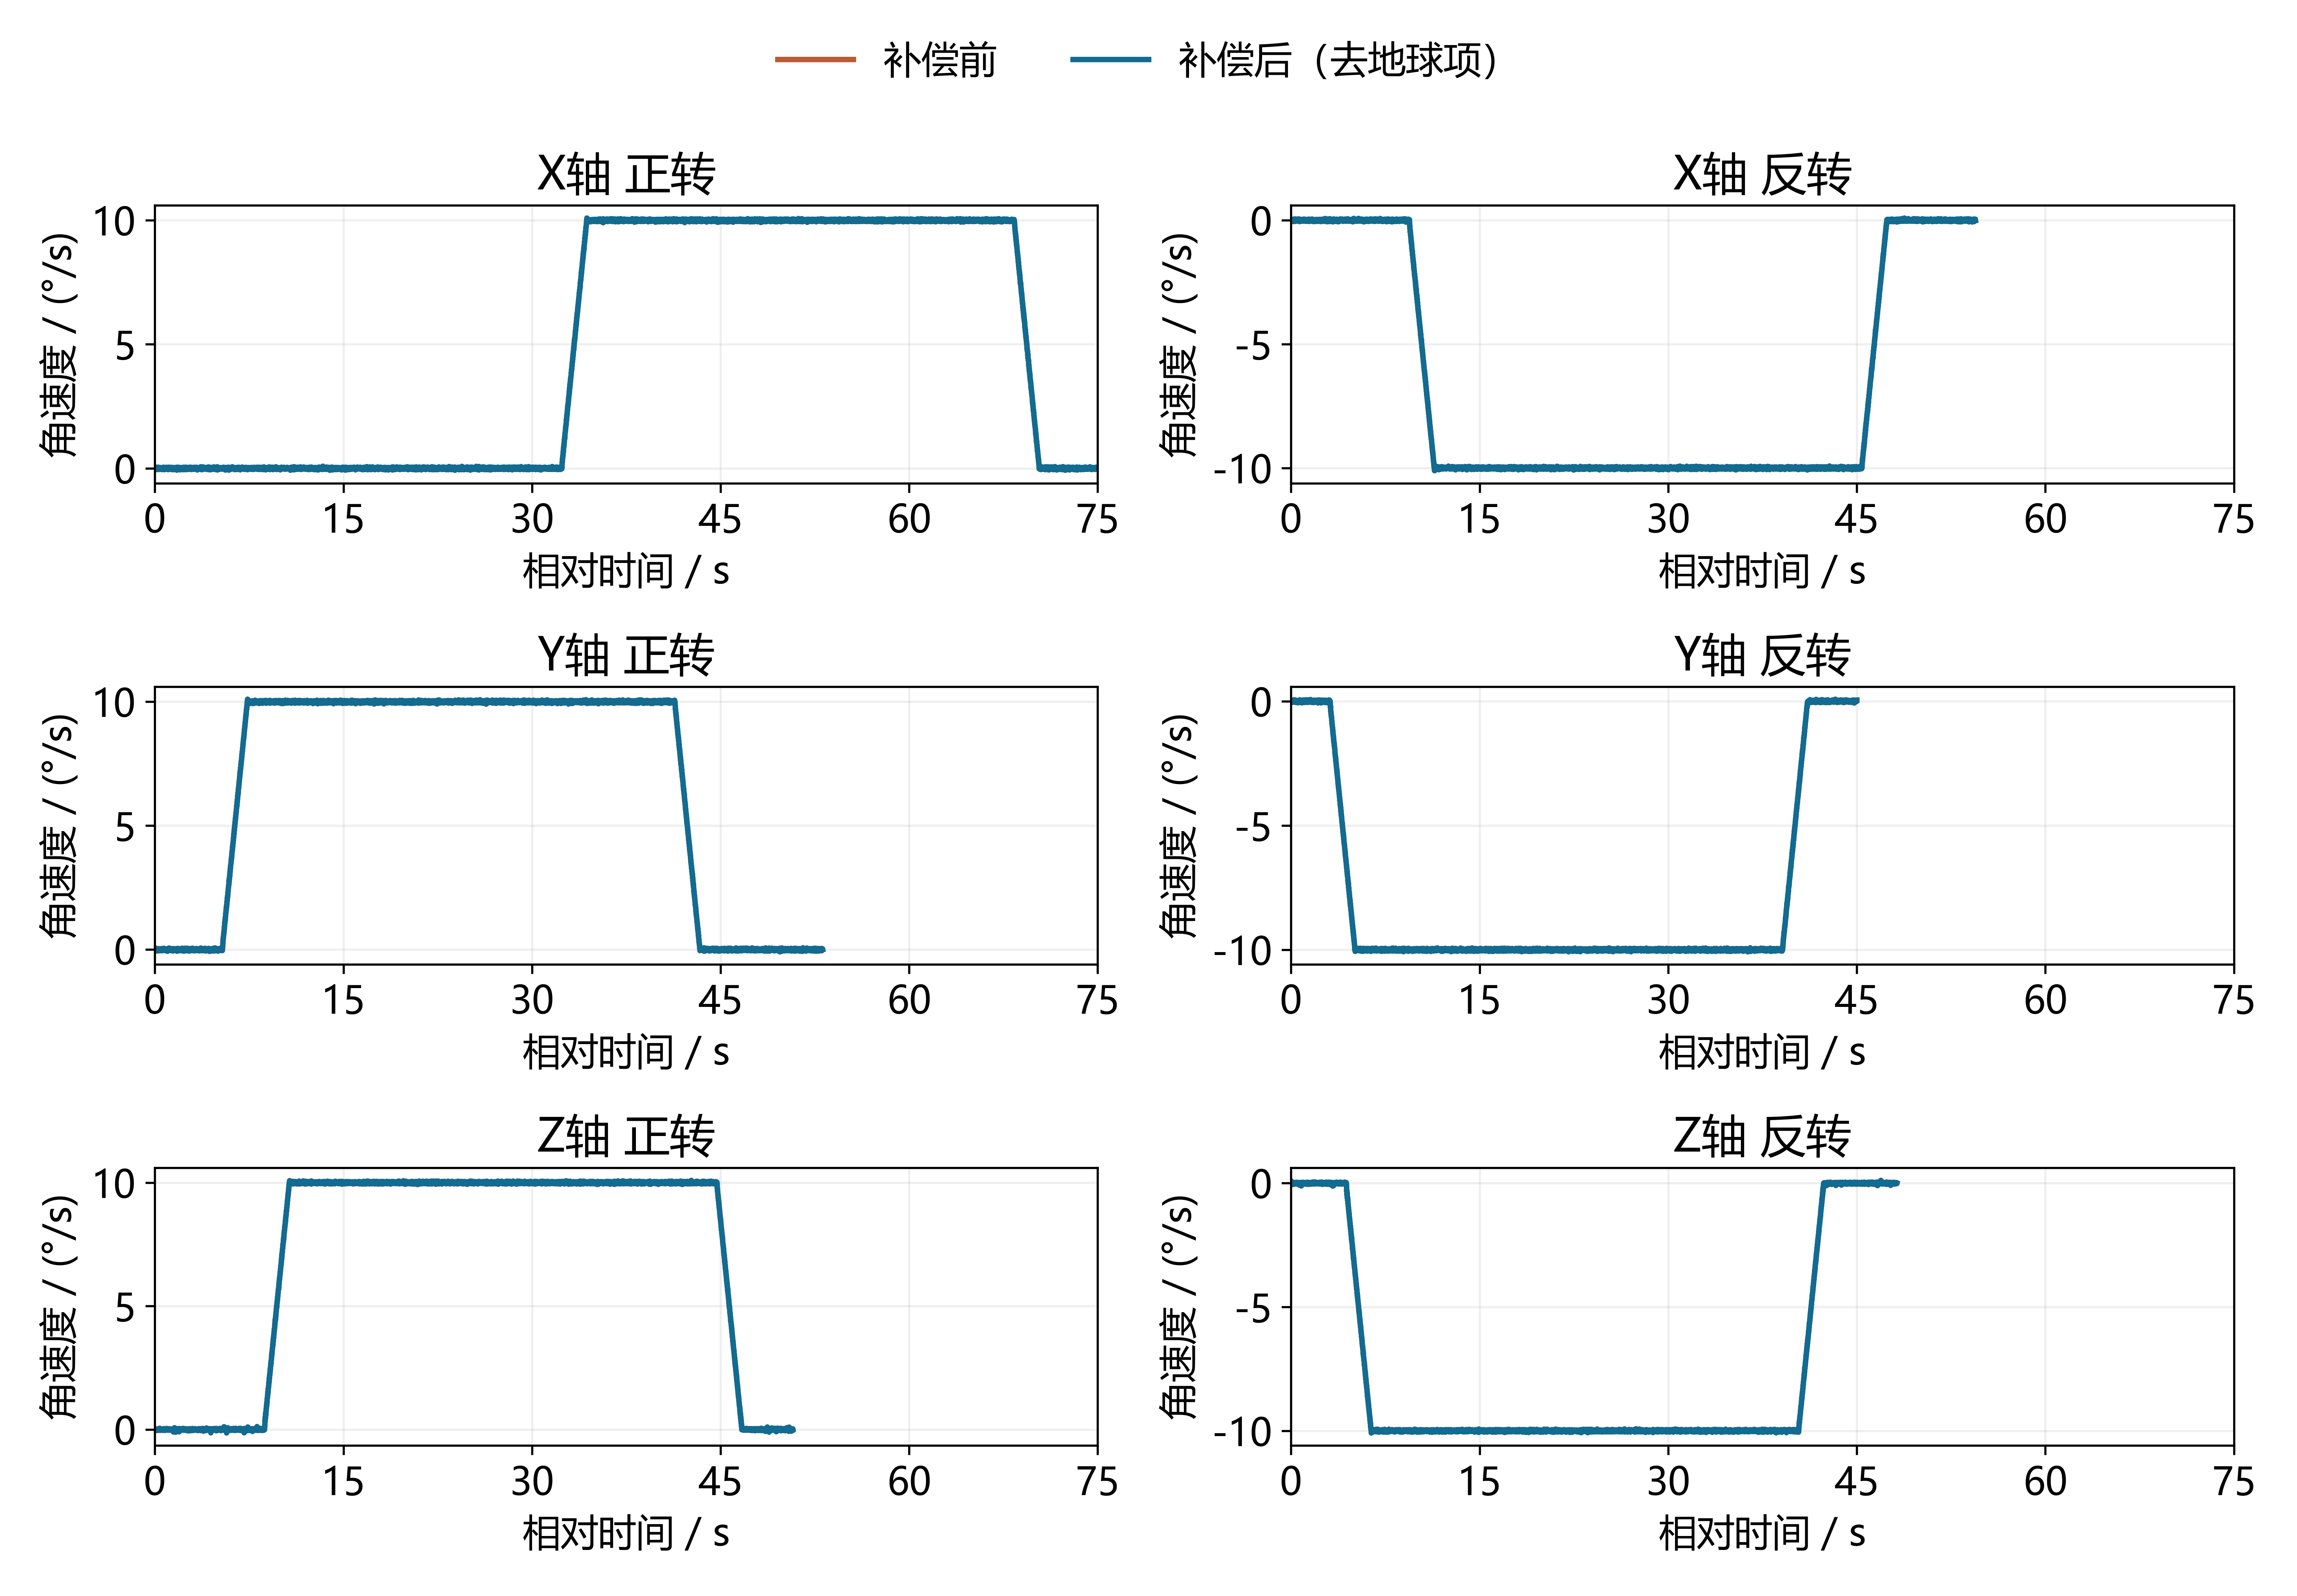
\includegraphics[width=1\textwidth]{gyro_compensation.png}
\caption{六次角速度补偿前后对比（0--75~s）}\label{fig:gyrocomp}
\end{figure}
图\ref{fig:gyrocomp}叠加原始角速度及去地球项后的转台角速度估计。两曲线在约$10^\circ$/s的平台上接近重合，误差相对主信号较小。表\ref{tab:gyroclosure}给出积分角与名义转角的差。


\begin{table}[htbp]\centering\small
\caption{转动积分角补偿前后闭合差}\label{tab:gyroclosure}
    \begin{tabular}{crrrr}\toprule
    转动&名义角/($^\circ$)&原始角差/($^\circ$)&补偿后转角/($^\circ$)&补偿后角差/($^\circ$)\\\midrule
    $X+$&360&-0.199994&360.012683&0.012683\\
    $X-$&-360&0.033808&-359.987317&0.012683\\
    $Y+$&360&-0.193917&360.015234&0.015234\\
    $Y-$&-360&0.069841&-359.984766&0.015234\\
    $Z+$&360&-0.238066&360.029928&0.029928\\
    $Z-$&-360&0.118380&-359.970072&0.029928\\\bottomrule
    \end{tabular}
\end{table}
补偿后绝对角差均下降，但正反转保留同号公共残差，分别约0.0127、0.0152、0.0299$^\circ$。比例因子由同一对转动差分估计，正反转差值闭合是代数上的必然结果。

静态数据也有模型偏离：上下均值半差在$X$、$Y$、$Z$轴分别为7.1035、7.0529、5.1112$^\circ$/h，而当地理论垂向地球自转约7.6411$^\circ$/h。尤其$Z$轴差异无法由约$-495$~ppm比例误差单独解释。可能涉及姿态不对称、交轴影响、温度或零偏变化。

\subsection{静态解析粗对准结果}

\begin{figure}[htbp]\centering
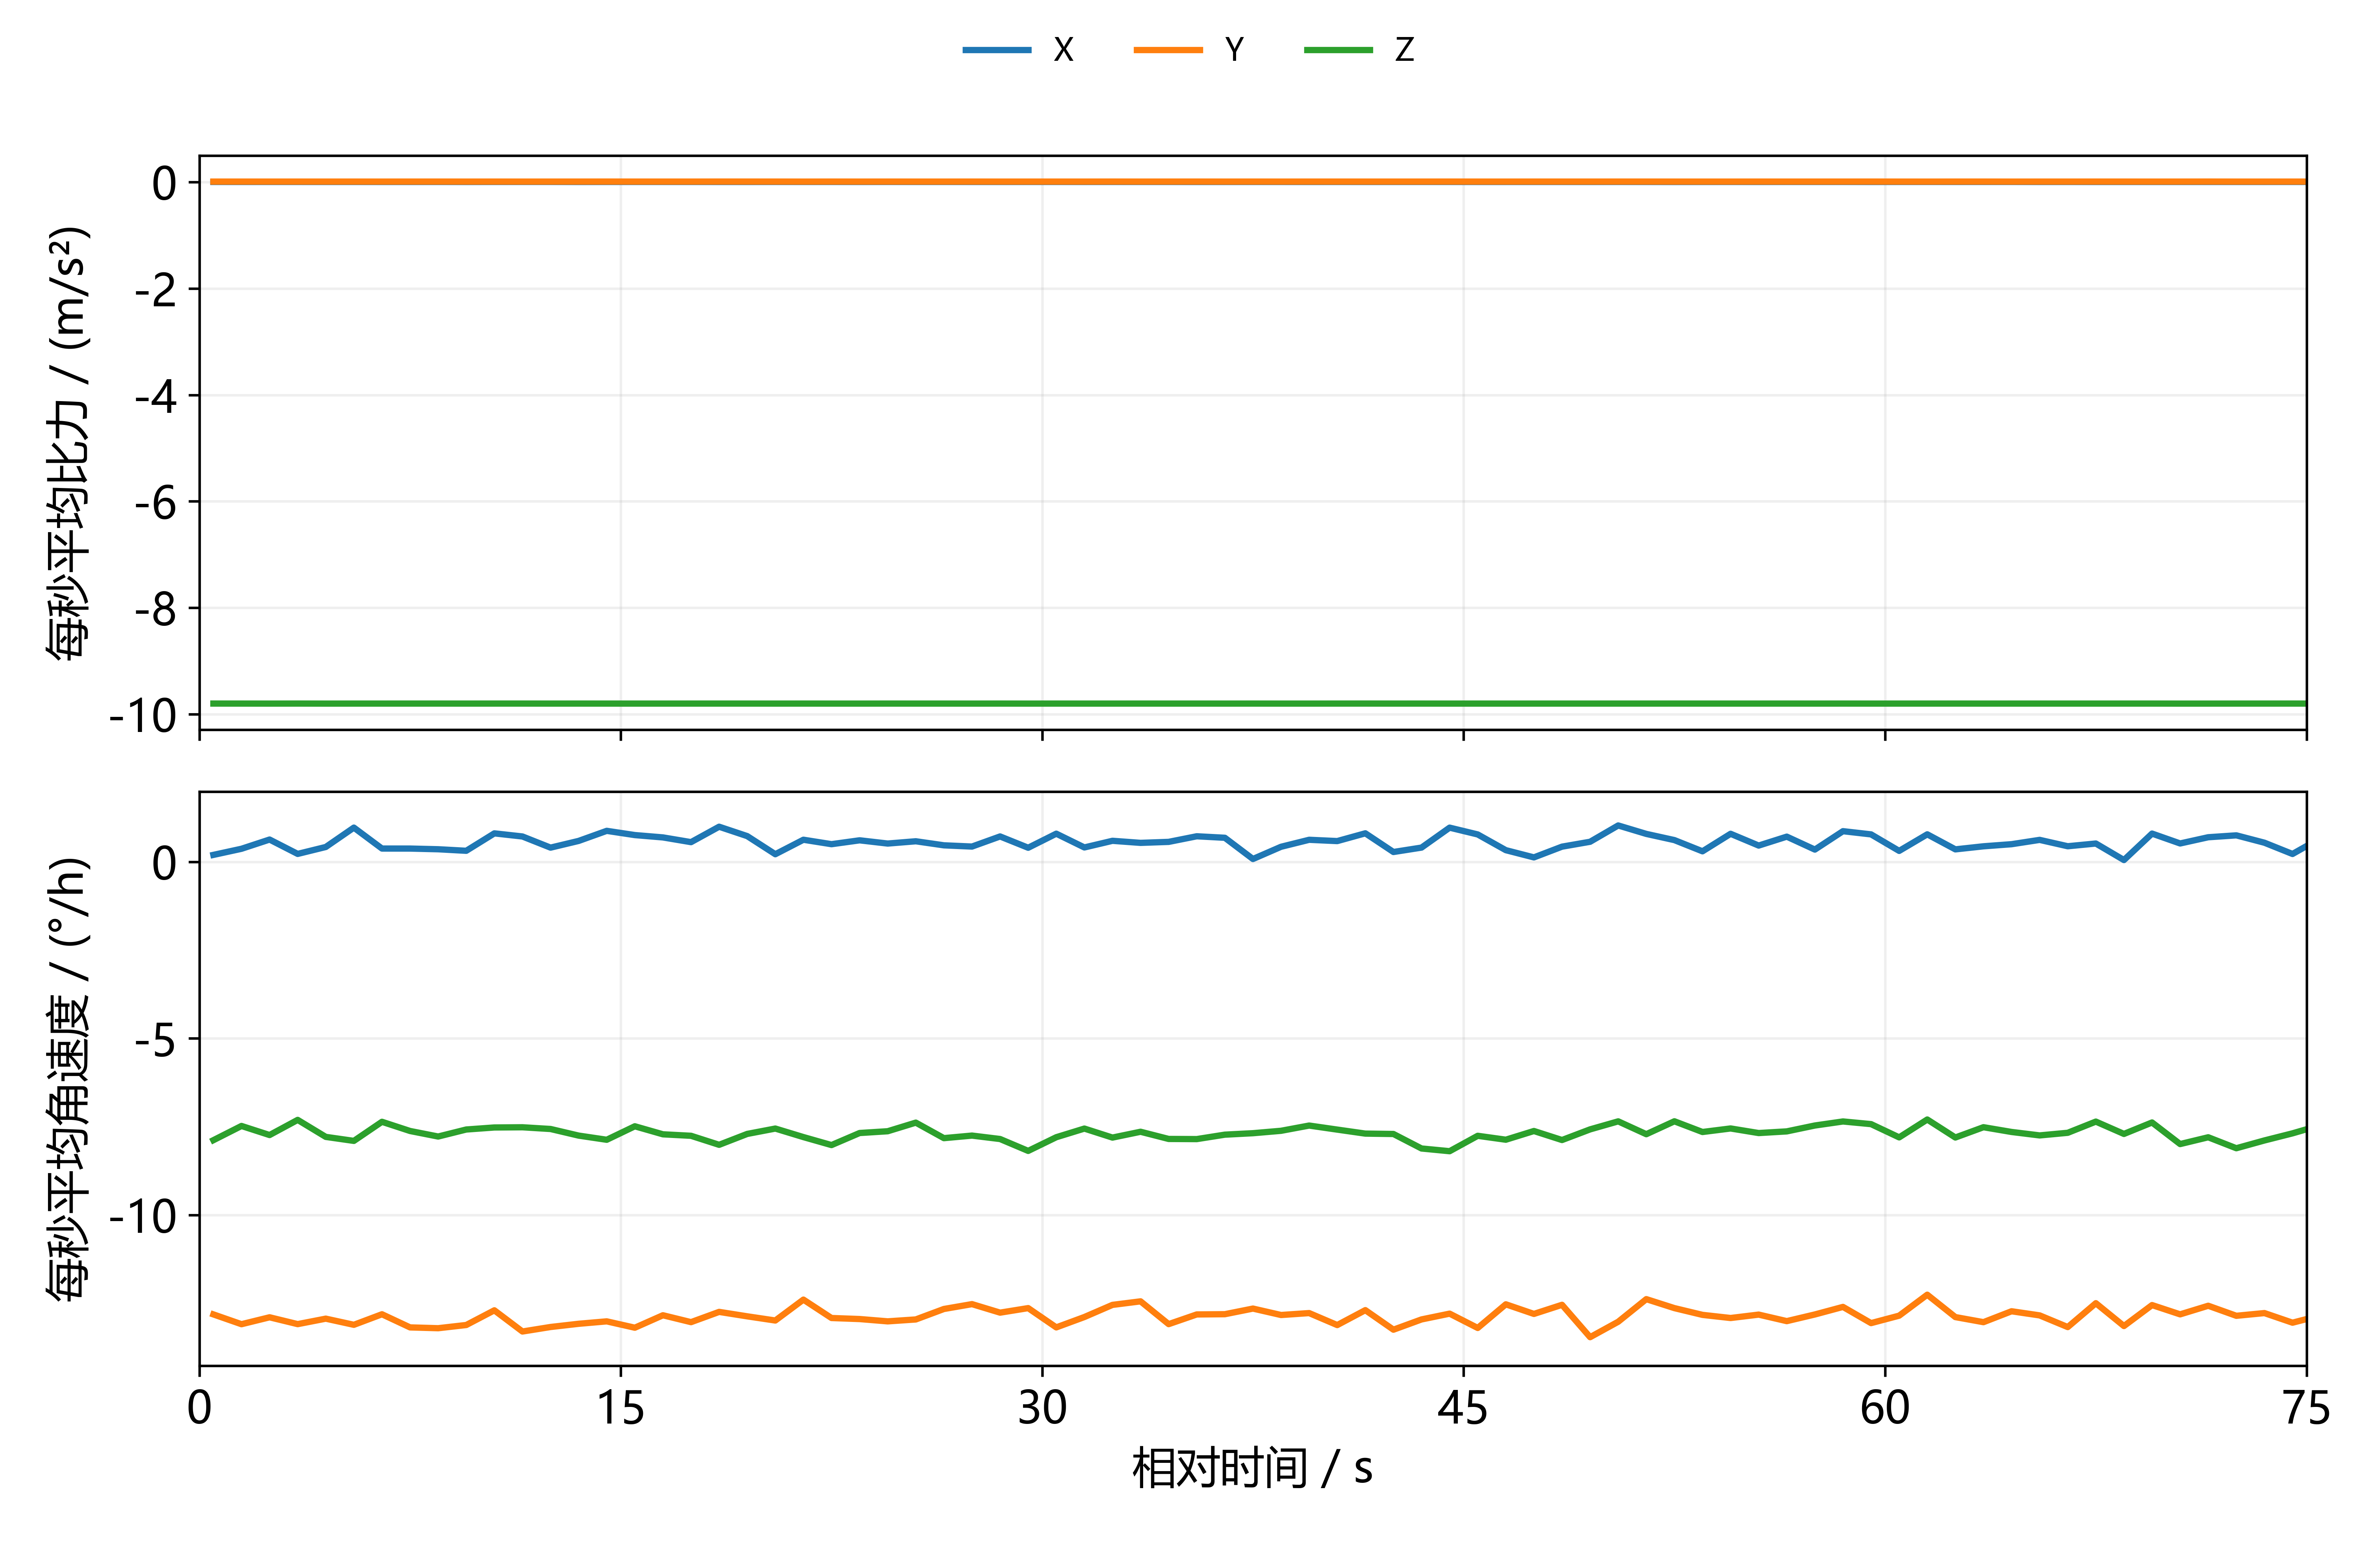
\includegraphics[width=0.85\textwidth]{alignment_observations.png}
\caption{100C静态观测前75~s的每秒平均比力和角速度}\label{fig:alignobs}
\end{figure}
图\ref{fig:alignobs}中$Z$比力接近$-9.8$~m/s$^2$，水平分量很小；角速度为地球自转投影与设备误差的共同结果。
\subsubsection{整段平均姿态}
平均观测为
\begin{equation}
\overline{\matr f}^{b}=\begin{bmatrix}-0.001196720\\0.005476272\\-9.797158599\end{bmatrix}~\mathrm{m/s^2},\qquad
\overline{\matr\omega}^{b}=\begin{bmatrix}2.5847901\\-62.3944531\\-37.1890022\end{bmatrix}10^{-6}~\mathrm{rad/s}.
\end{equation}
所得矩阵
\begin{equation}
\matr C_b^n=\begin{bmatrix}
0.041449869&-0.999140426&-0.000563548\\
0.999140577&0.041449931&-0.000098876\\
0.000122150&-0.000558965&0.999999836
\end{bmatrix}.
\end{equation}
未舍入矩阵检验：$\|\matr C_b^n(\matr C_b^n)^T-\matr I\|_F<10^{-12}$，行列式与1之差小于$10^{-12}$，满足正交性和右手性。
\begin{table}[htbp]\centering
\caption{整段观测的解析粗对准结果}\label{tab:whole}
\begin{tabular}{ccc}\toprule
航向$\psi$/($^\circ$)&俯仰$\theta$/($^\circ$)&横滚$\phi$/($^\circ$)\\\midrule
87.624417&-0.006999&-0.032026\\\bottomrule
\end{tabular}\end{table}
设备$X$轴水平投影大致朝东，设备接近水平。小数位用于数值复现，不表示达到相同绝对精度。没有独立姿态真值，整段解仅作内部比较基准。

\subsubsection{每秒与逐历元姿态}
\begin{figure}[htbp]\centering
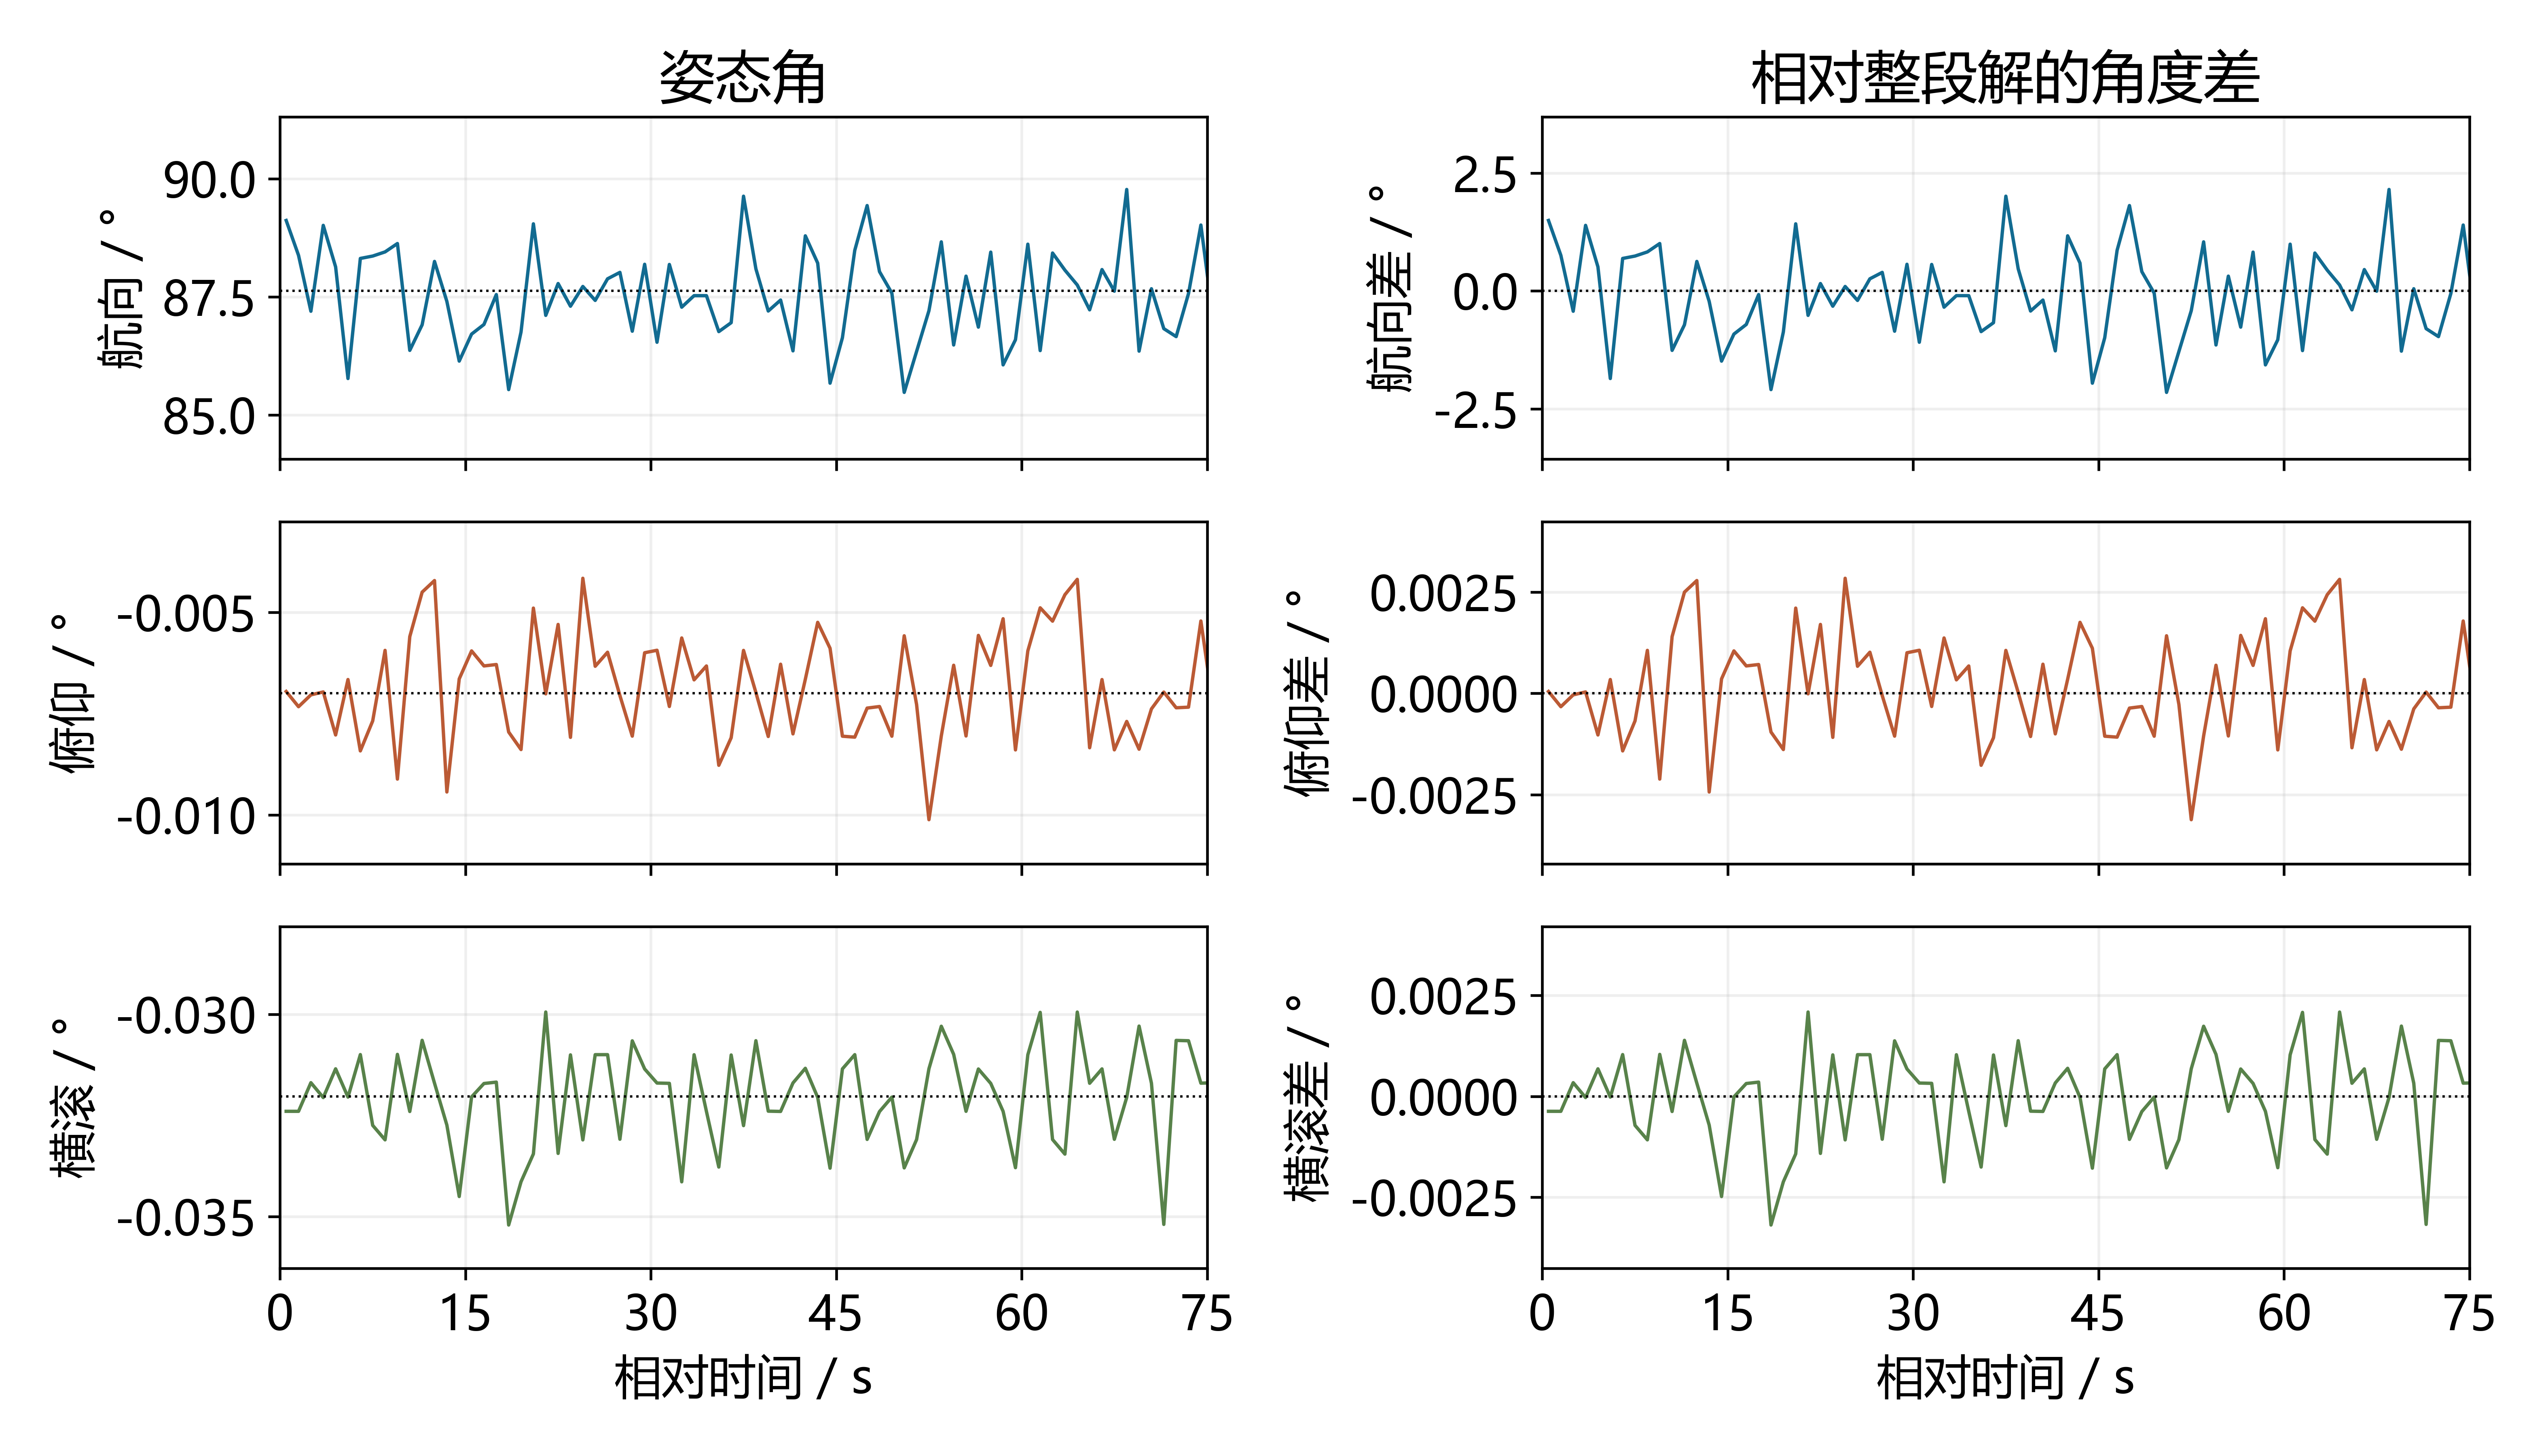
\includegraphics[width=0.85\textwidth]{alignment_second.png}
\caption{每秒平均姿态及相对整段解的角差（0-75~s）}\label{fig:second}
\end{figure}

图\ref{fig:second}给出前75~s的每秒平均姿态，其中航向角差归化到$[-180^\circ,180^\circ)$，避免把角度跨界误记为接近$360^\circ$的误差。图\ref{fig:second}表明每秒平均后的水平姿态集中在整段结果附近，航向仍有约度级起伏。平均能改善地球自转方向估计，但航向对弱信号误差仍比俯仰、横滚敏感。图\ref{fig:epoch}和图\ref{fig:epochhist}分别从时序变化和分布密集程度两个角度展示同一时段的逐历元解,整段基准姿态和表中统计量仍由完整记录计算。

\begin{figure}[htbp]\centering
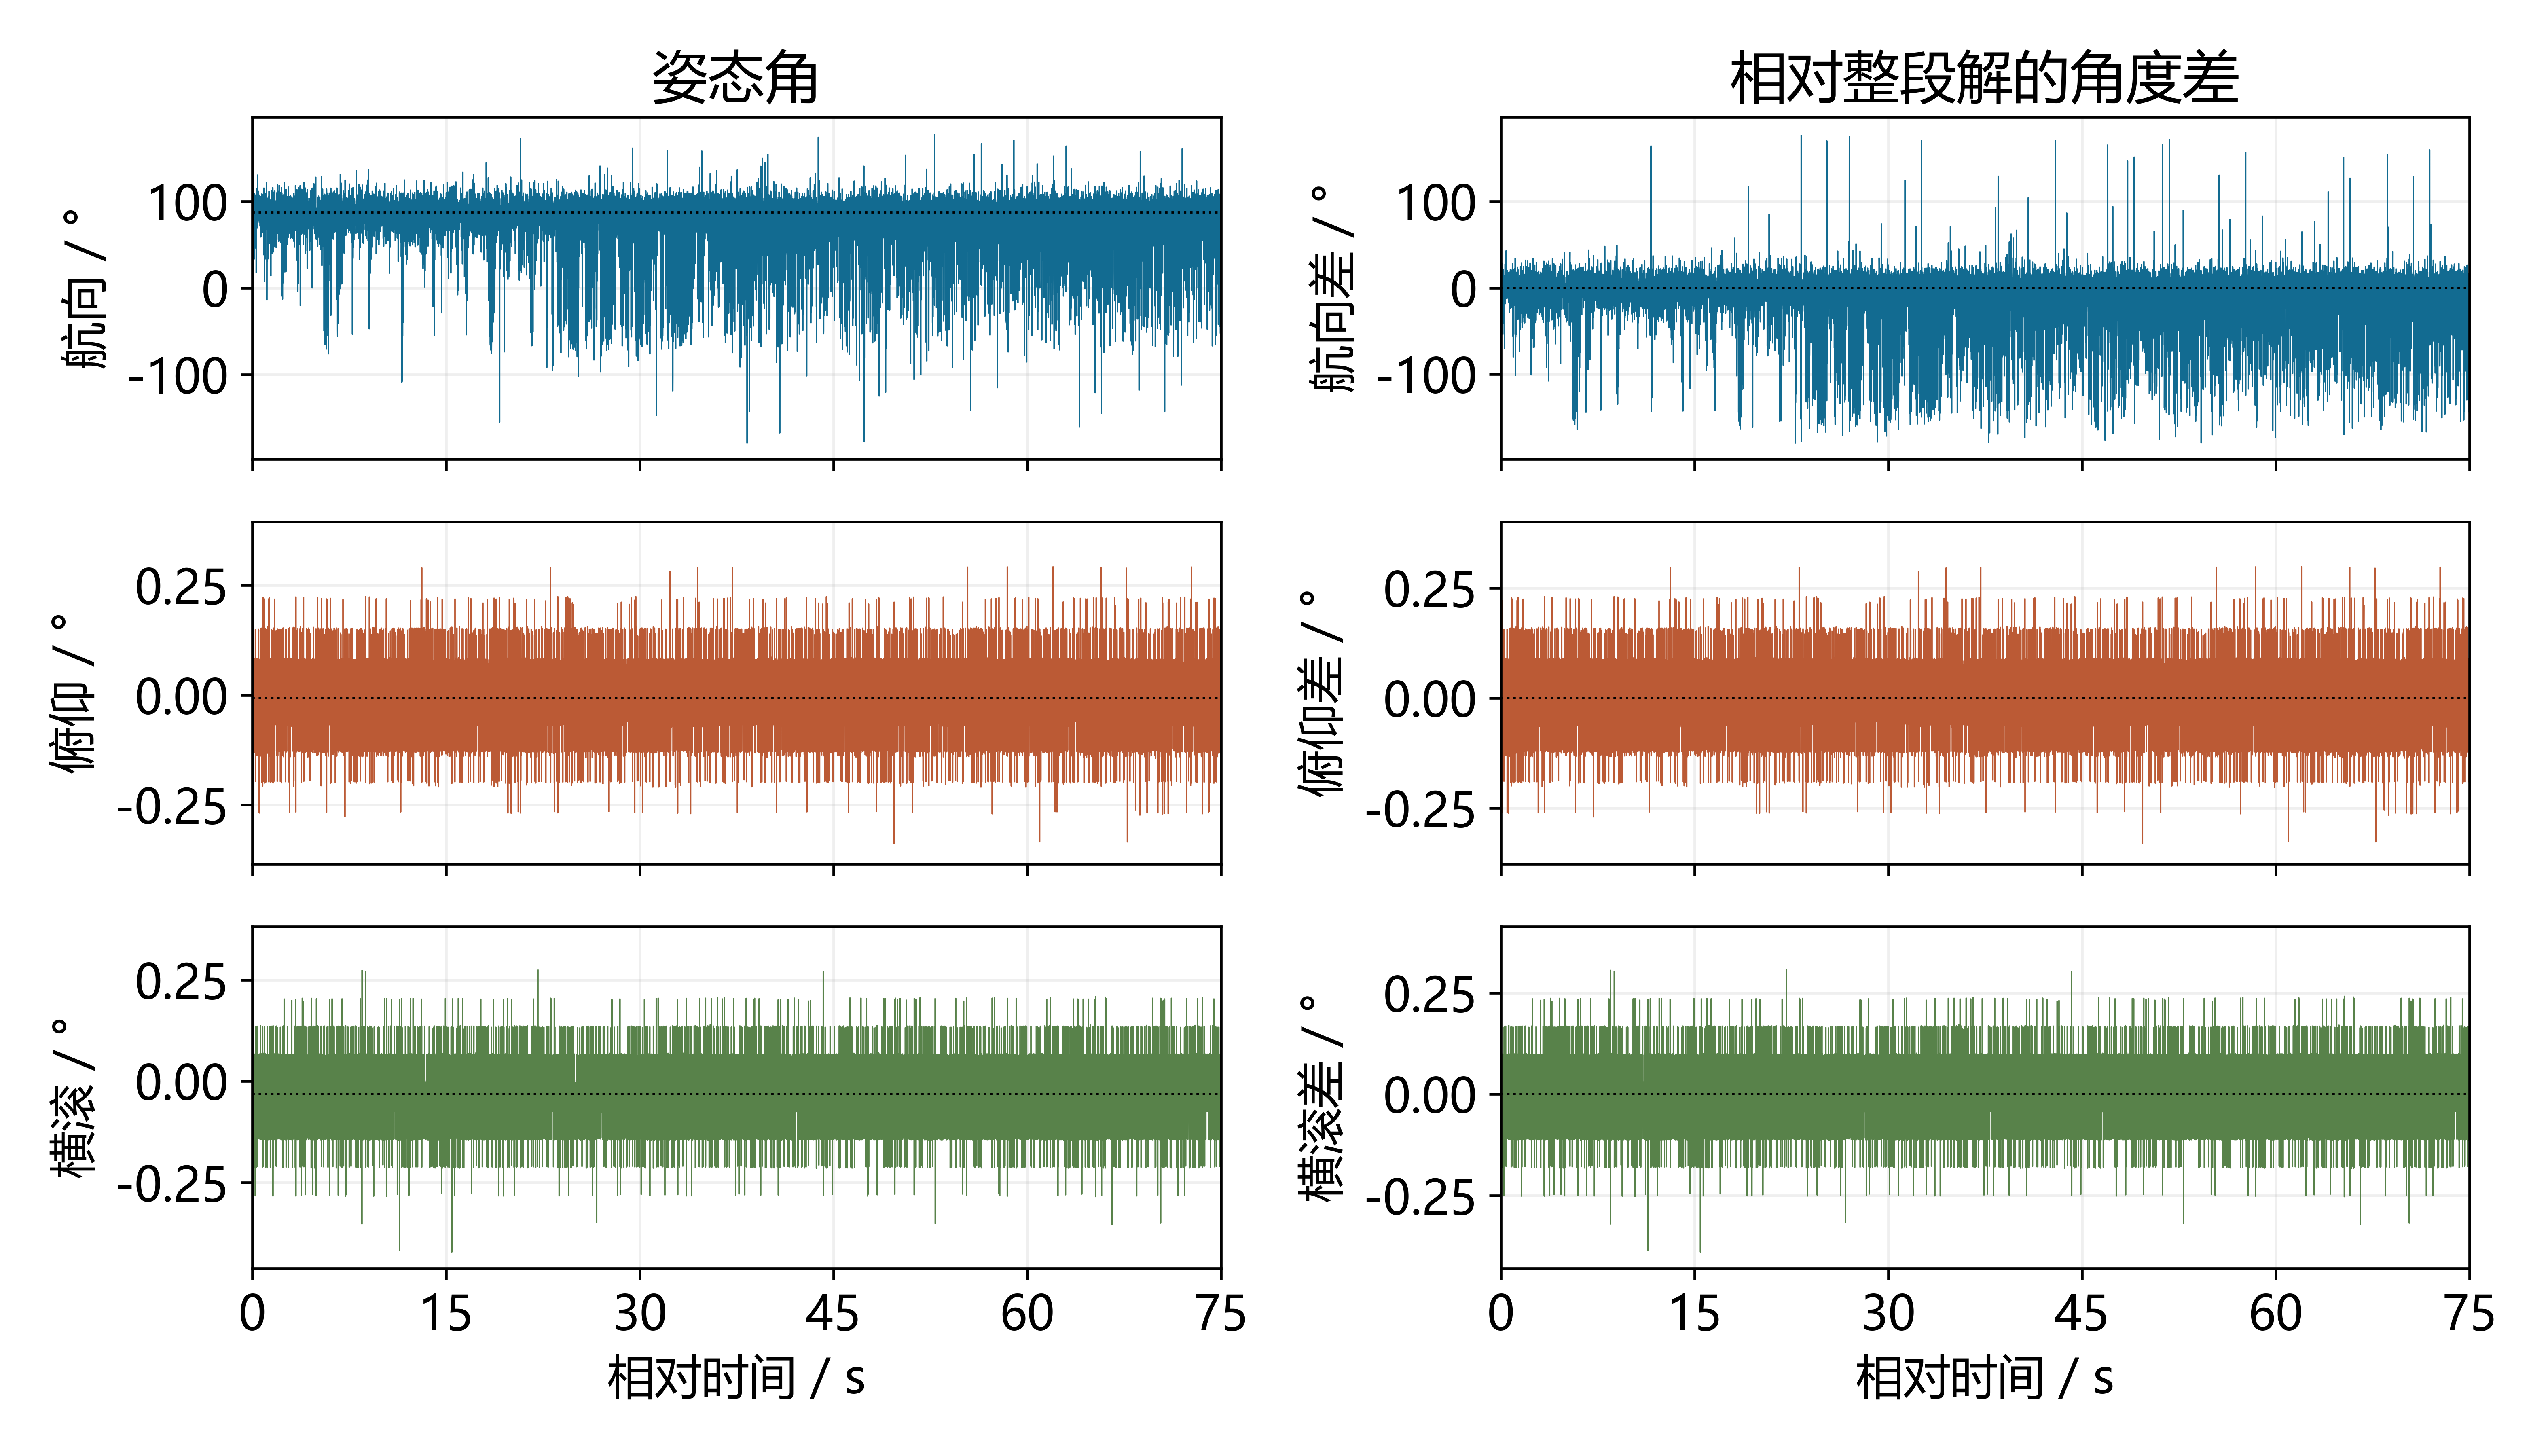
\includegraphics[width=0.85\textwidth]{alignment_epoch.png}
\caption{逐历元姿态及相对整段解的角差时序（0-75~s）}\label{fig:epoch}
\end{figure}
图\ref{fig:epoch}左列为航向、俯仰和横滚，右列为对应的归化角差，水平点线分别标记整段姿态和零差值。单历元航向起伏远大于俯仰、横滚，说明5~ms观测下地球自转方向估计易受噪声影响。连线仅表示相邻解的时间顺序，密集尖峰不能解释为设备的真实连续转动；分布密集程度见图\ref{fig:epochhist}。


\begin{figure}[htbp]
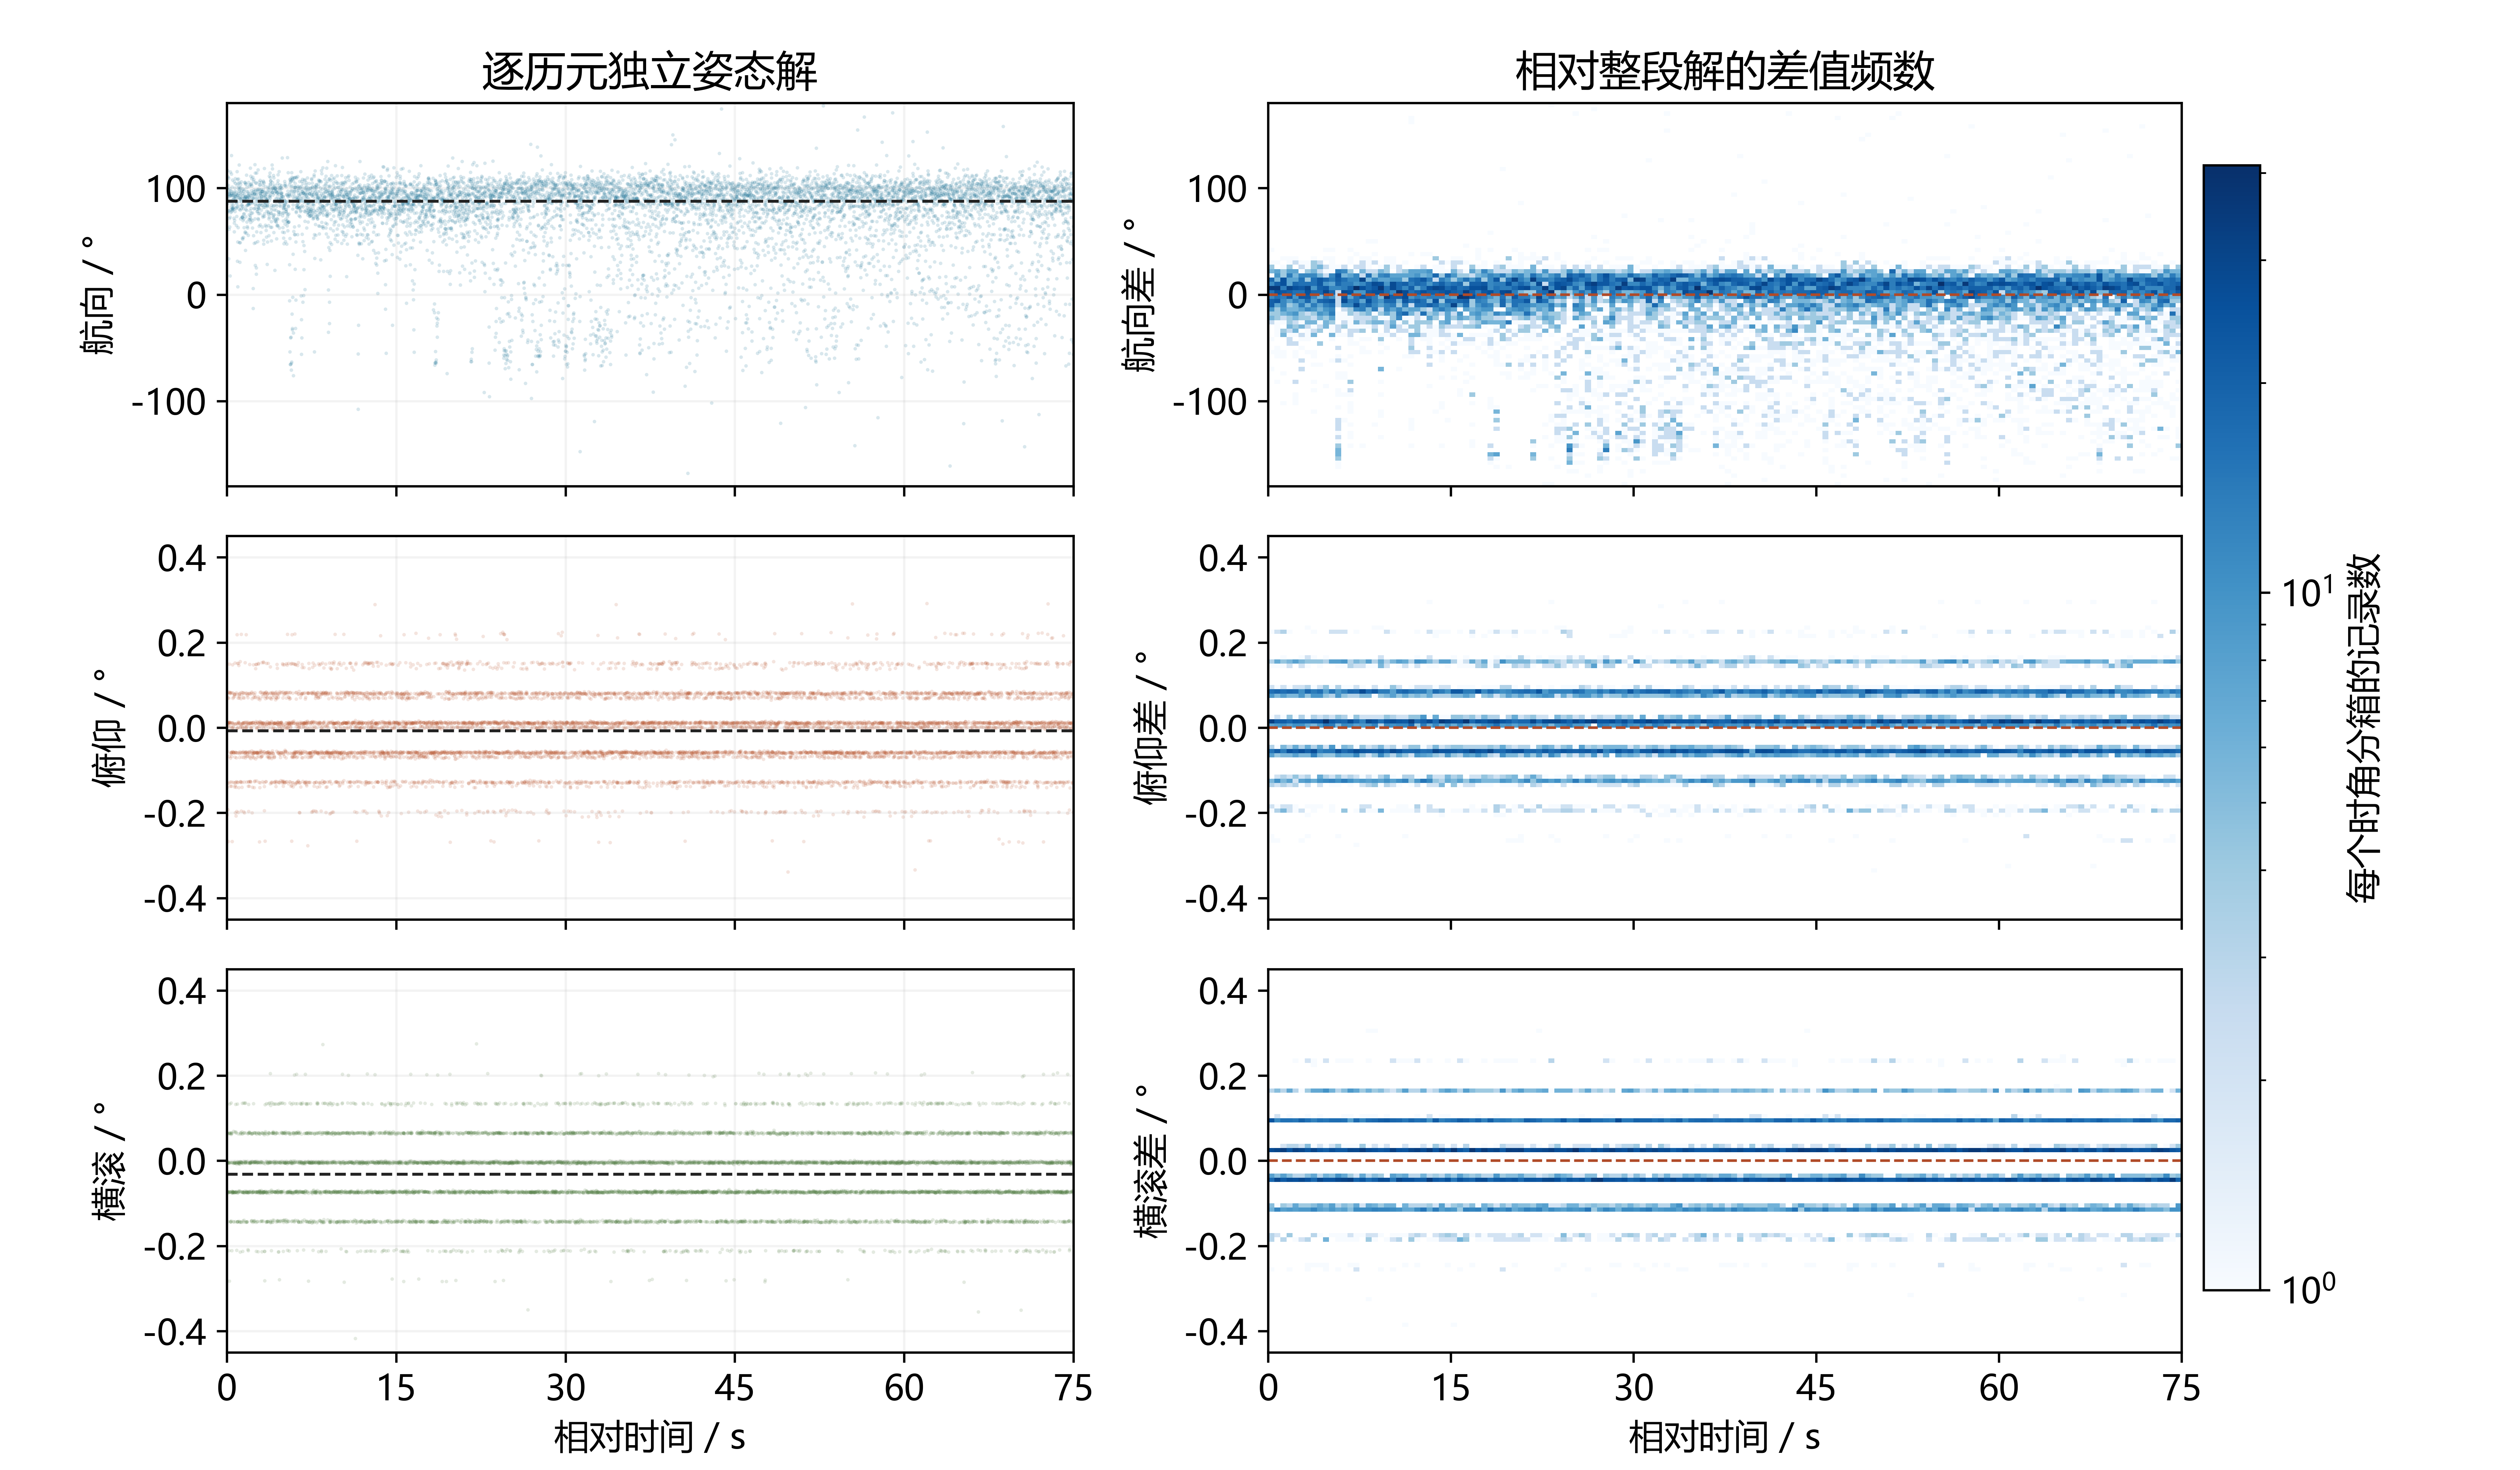
\includegraphics[width=1\textwidth]{alignment_epoch_his.png}
\caption{逐历元姿态散点与相对整段解的时角二维频数（0-75~s）}\label{fig:epochhist}
\end{figure}
图\ref{fig:epochhist}左列每隔一个样本绘制一个散点，黑色虚线为整段姿态；右列使用该时段全部样本，按0.5~s时间窗及角差区间统计频数，红色虚线为零差值。各子图内蓝色越深表示记录越密集，采用对数色阶。航向存在远离密集区的样本，俯仰、横滚呈较窄的水平条带，散点和频数图使连线遮蔽的分布结构更清楚。


\FloatBarrier
\begin{table}[htbp]\centering\small
\caption{相对整段解的RMS差与最大绝对差（$^\circ$）}\label{tab:alignstats}
\begin{tabular}{llrrr}\toprule
方式&指标&航向&俯仰&横滚\\\midrule
逐历元&RMS差&43.777405&0.086338&0.085160\\
逐历元&最大绝对差&179.988150&0.366079&0.391581\\
每秒平均&RMS差&0.978794&0.001152&0.001191\\
每秒平均&最大绝对差&3.358429&0.003851&0.003877\\\bottomrule
\end{tabular}\end{table}
统计定义
\begin{equation}
\operatorname{RMS}_{\Delta\alpha}=\sqrt{\frac1N\sum_{k=1}^{N}
\left[\operatorname{wrap}_{180}(\alpha_k-\alpha_{\rm all})\right]^2}.
\end{equation}

每秒平均将航向RMS差从43.777$^\circ$降到0.979$^\circ$，约缩小44.7倍；俯仰和横滚分别约缩小75.0、71.5倍。单历元航向最大差接近180$^\circ$，说明单周期内地球自转水平分量易受噪声干扰，非线性定姿又放大方向不稳定性。重力信号强于地球自转，因此水平姿态稳定得多。

\subsubsection{平均时长的影响}
小误差量级关系为
\begin{equation}
\delta\theta,\delta\phi\sim b_{a,h}/g,\qquad
\delta\psi\sim b_{g,E}/(\Omega\cos L).
\end{equation}
当地地球自转水平分量约12.9555$^\circ$/h。取名义零偏0.05$^\circ$/h，其对应的航向误差量级为0.2211$^\circ$；分别取角随机游走（ARW）为0.005和0.012$^\circ$/\(\sqrt{\mathrm{h}}\)，平均1800~s后的白噪声航向量级约为0.0313$^\circ$和0.0751$^\circ$。

\begin{figure}[htbp]\centering
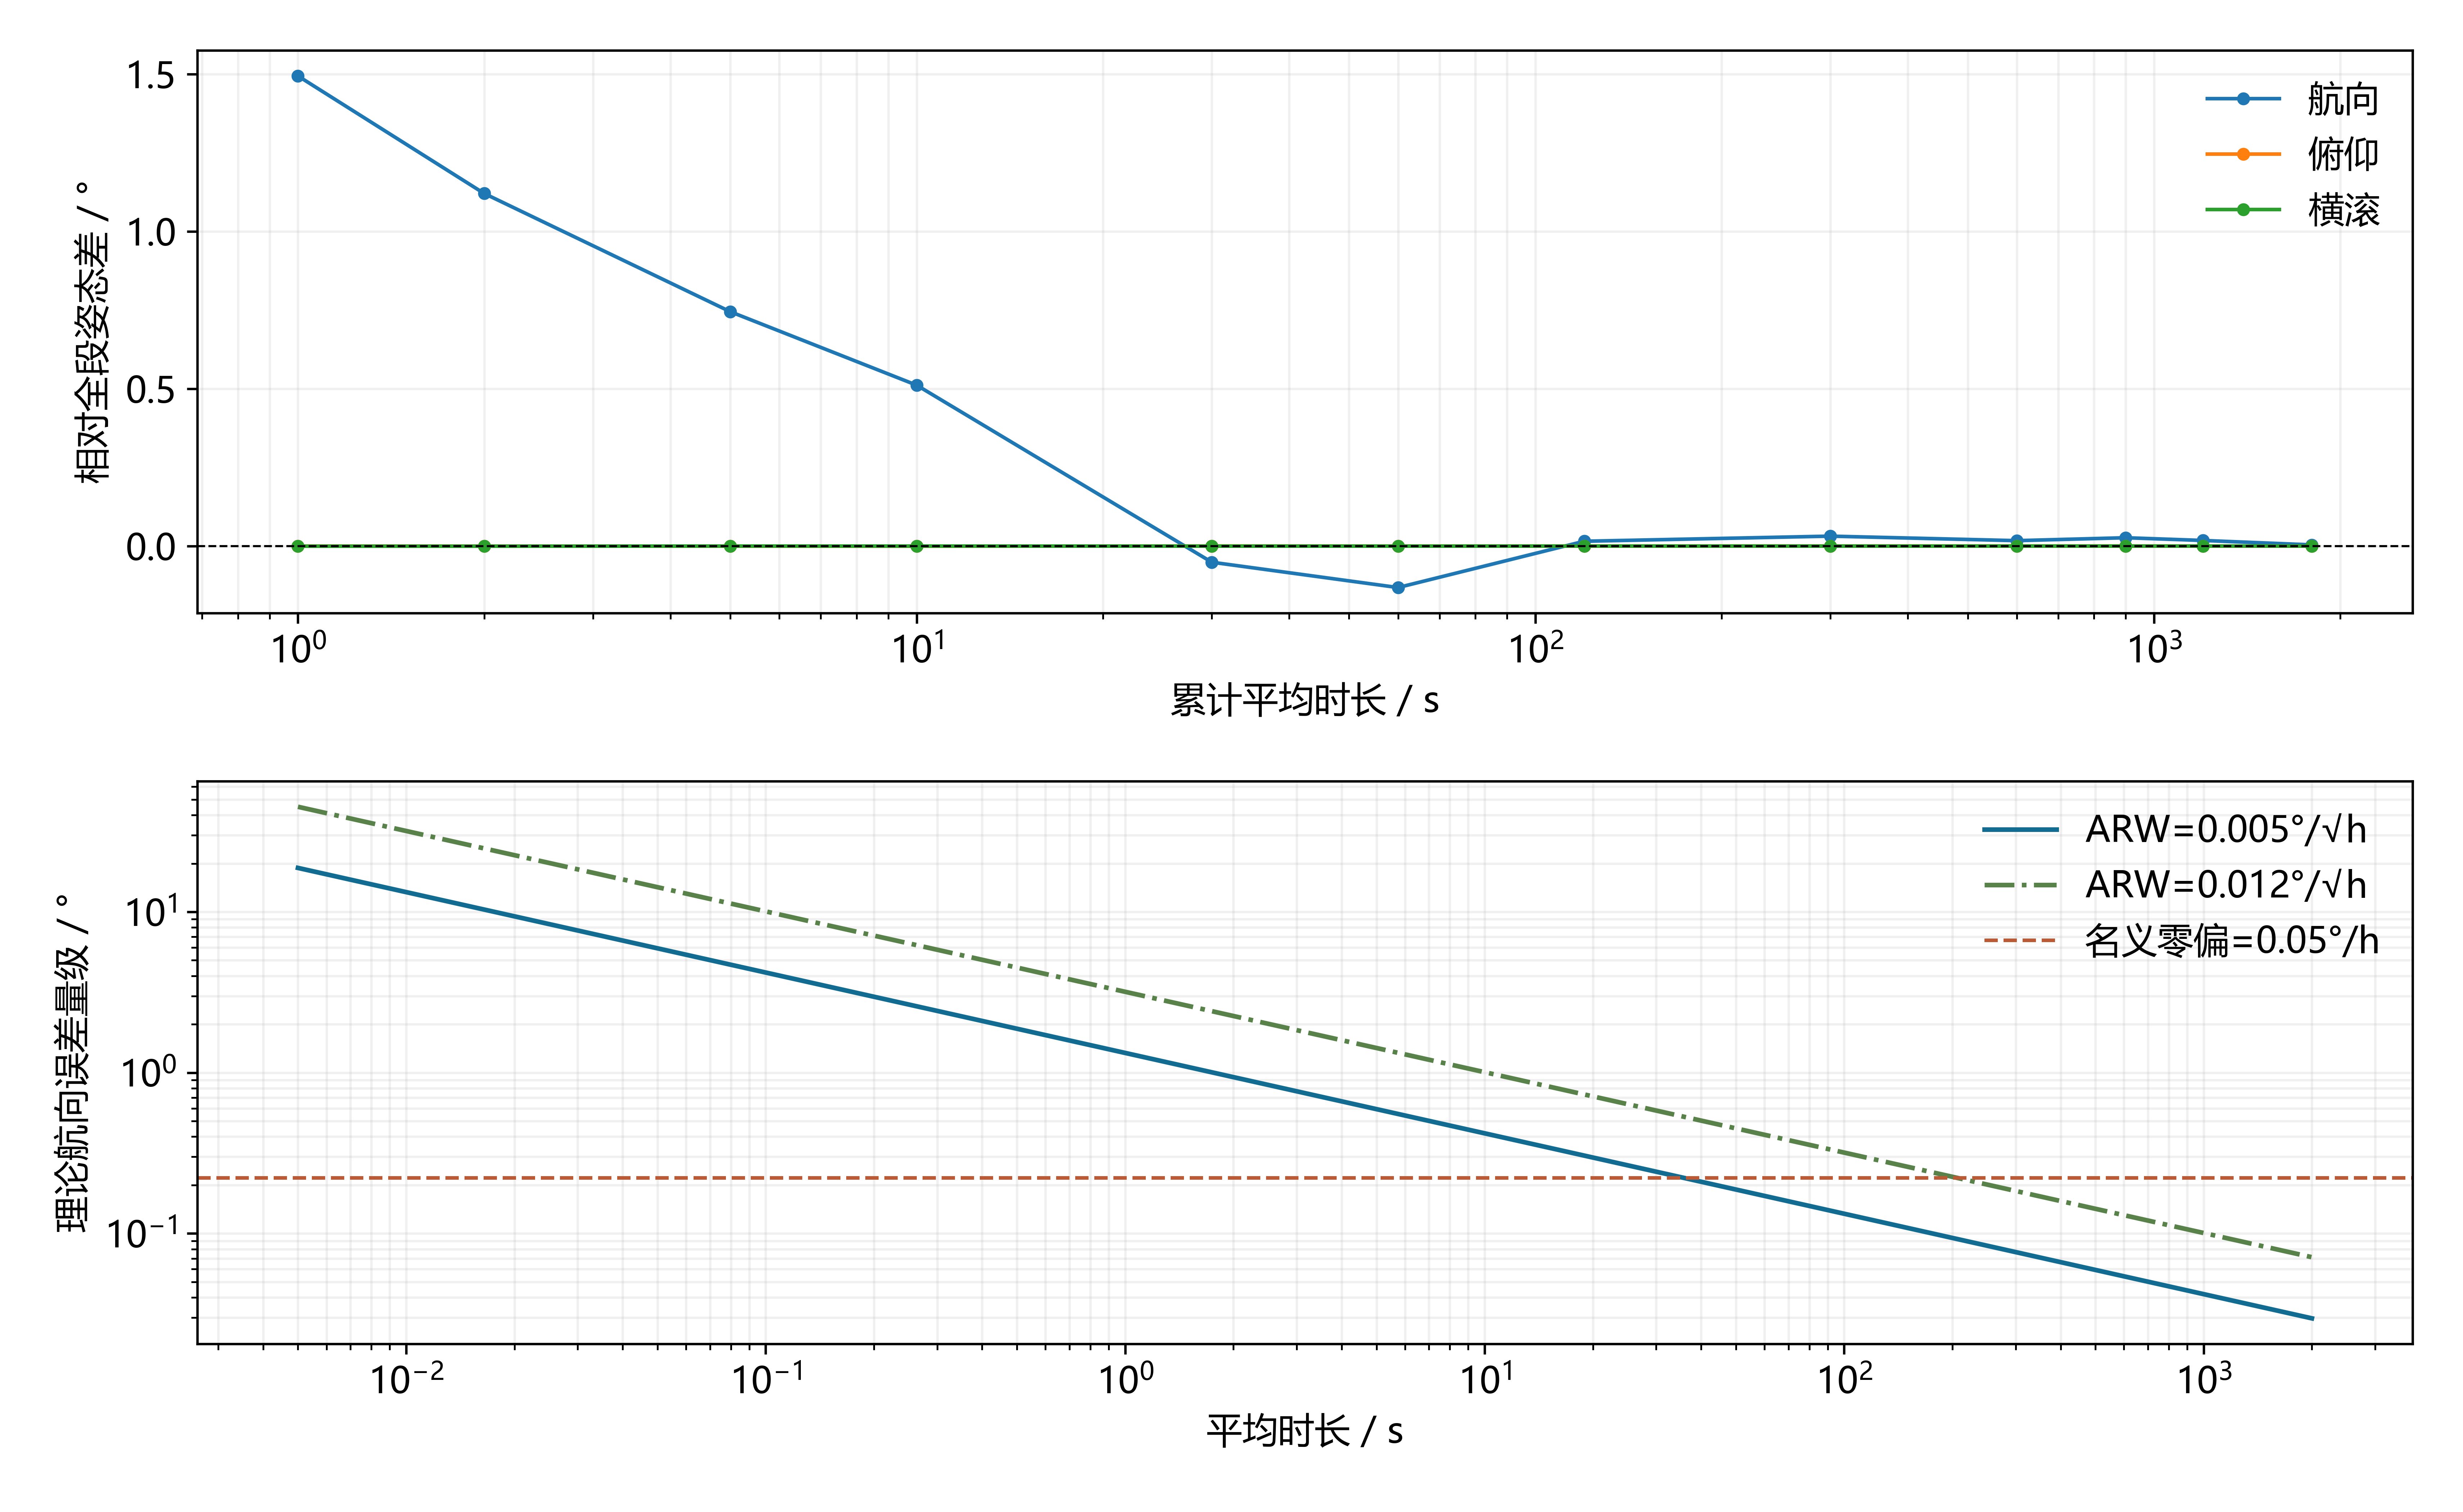
\includegraphics[width=0.85\textwidth]{alignment_averaging_his.png}
\caption{累计平均姿态变化与两种ARW假设下的理论航向误差量级}\label{fig:average}
\end{figure}
图\ref{fig:average}左侧采用对数时间轴，累计平均航向总体趋近整段解，但局部并不单调；俯仰、横滚在同一纵轴尺度下接近零线。右侧两条斜线分别对应两种ARW假设，独立白噪声的航向量级随$T^{-1/2}$衰减，较大ARW对应较大误差；水平虚线表示固定零偏的影响不会随平均时间消失。右图为小误差近似下的理论量级，短时大角差区仅作趋势参考。
\begin{table}[htbp]\centering\small
\caption{代表性累计平均时长的航向结果}
\begin{tabular}{rrr}\toprule
时长/s&航向/($^\circ$)&相对全段差/($^\circ$)\\\midrule
1&89.118304&1.493887\\10&88.135790&0.511373\\30&87.573136&-0.051281\\
60&87.492646&-0.131771\\120&87.639776&0.015359\\300&87.656012&0.031595\\
600&87.641699&0.017282\\1800&87.628285&0.003868\\\bottomrule
\end{tabular}\end{table}
平均时间增长后总体接近全段解，但不逐步单调改善，例如30到60~s的差绝对值增大。白噪声衰减、低频变化和有限样本波动共同作用。

